\documentclass[12pt,a4paper]{article}
\usepackage[a4paper,left=27mm,right=27mm,top=27mm,bottom=27mm]{geometry}
\linespread{1.23}
\usepackage{amsmath,amssymb,booktabs,tabularx,longtable,array,graphicx,hyperref,url,xurl,enumitem,caption}
\usepackage{float}
\usepackage{makecell,adjustbox,multirow,siunitx,algorithm,algpseudocode,subcaption}
\usepackage[numbers,sort&compress]{natbib}
\setlength{\emergencystretch}{5em}
\sloppy
\newcolumntype{Y}{>{\raggedright\arraybackslash}X}
\newcolumntype{C}{>{\centering\arraybackslash}X}
\newcommand{\mtt}[1]{\texttt{#1}}
\newcommand{\RepoURL}{https://github.com/ErcanErkalkan/AI_Enabled_Standards_Aligned_Security_Risk_Management}
\newcommand{\repo}{\url{\RepoURL}}
\newcommand{\RepoLink}{\href{\RepoURL}{the project repository}}
\newcommand{\NVDfeed}{\textsc{NVD} CVE API~2.0 / local CVSS cache}
\newcommand{\NVDfeeds}{\textsc{NVD} CVE API~2.0 / local CVSS caches}
\newcommand{\R}{\mathrm{R}}
\title{Control-Scoped Evidence-First GQM for Security Standards Traceability: A Bounded Question-Repair and UML/XMI Evaluation}
\author{Ercan Erkalkan\\\small Marmara University, Istanbul, Turkey\\\small \texttt{ercan.erkalkan@marmara.edu.tr}\\\small ORCID: 0000-0001-9259-7112}
\date{}
\begin{document}
\maketitle
\begin{abstract}
\noindent\textbf{Context:} Model-driven compliance tools represent controls, traces and evidence, but evidence-specific questions can inadvertently prescribe obligations beyond the source control. \textbf{Objective:} This study evaluates control-scoped GQM question wording and targeted repair in a bounded archival artifact assessment. \textbf{Method:} A 199-control catalogue supports a fixed 24-task primary comparison, a separate four-task exploratory set and targeted repair of 15 previously flagged controls. UML/XMI, mapping and historical telemetry results provide supporting evidence. The identity and authorization of the recorded scorers have not been independently verified. \textbf{Results:} Across the 24 primary tasks, mean actionability increased from 2.00 to 4.17/5 and mean semantic fidelity changed from 3.94 to 3.63, with 23/48 unsupported-prescription flags. In the selected repairs, mean fidelity increased from 2.97 to 4.87; a post-hoc joint quality criterion was met for 1/30 original and 30/30 revised scorer-presentations, not independent controls. \textbf{Conclusion:} Specificity and source-control scope can diverge. The observed selected-case repairs illustrate a traceable way to constrain evidence requests, without establishing causal superiority, population-wide effectiveness or field generalizability.
\end{abstract}
\noindent\textbf{Keywords:} Evidence-first GQM; standards traceability; UML/XMI; security evidence; structural validation; semantic scope.\par\medskip
\section{Introduction}
Security evidence management is a software-engineering problem as well as an assurance problem: teams must preserve a reviewable connection from a versioned normative source and a particular control to the question asked, the record inspected, the responsible source, and the outcome of a validation run. Traceability research has long recognized the difficulty of maintaining such links across evolving artifacts~\cite{Gotel1994Traceability,RameshJarke2001Traceability}. Model-based compliance, reusable metamodels, assurance evidence lifecycles, and the NIST Open Security Controls Assessment Language (OSCAL) address closely related needs~\cite{PanesarWalawege2013IST,DelaVara2016IST,DelaVara2022SoSyM,NIST_OSCAL_2026}. Neither UML modeling nor evidence linkage is claimed to be new.

\noindent\textbf{Source-supported motivation and unmeasured burden.}
The practical concern is a potential \emph{review error}, not an observed prevalence estimate: a record request may be easy to execute yet require obligations that the cited control does not impose. Prior industrial compliance and evidence-lifecycle research documents the relevance of change impact, evidence completeness and human interpretation~\cite{DelaVara2022SoSyM,Nair2015IST}; GQM provides a disciplined connection from measurement goals to questions~\cite{Basili2014GQM}, while OSCAL already supports machine-readable assessment records~\cite{NIST_OSCAL_2026}. These sources motivate the mechanism, but none supplies a measured occurrence rate or monetary cost for the specific GQM question-overreach defect evaluated here. The present study consequently measures the defect \emph{inside its selected assessment tasks}, not its prevalence, auditor-hours lost, remediation expense or enterprise-wide compliance impact. A cost claim would require a separate prospective, time-logged practitioner study.

The research problem is a measurable failure mode of evidence-question operationalization: adding concrete record types can increase actionability while silently importing requirements from neighbouring controls. This study examines whether control-scoped revision of such questions restores \emph{joint} semantic fidelity, actionability, provenance and absence of unsupported prescriptions. Goal--Question--Metric (GQM) supplies the question structure~\cite{Basili2014GQM}; the contribution tested here is the documented error--repair contrast, not the invention of GQM, trace links, or a new compliance metamodel. The 24-task primary assessment and 15 selected repairs are separate analyses, not an externally controlled superiority experiment.

The \emph{single primary research question} (RQ) is: \emph{How does evidence-question specificity affect control-scope fidelity and actionability, and what changes after targeted repair of previously flagged questions?} Three supporting evaluation checks establish the artifact's scope, not further novel research questions: \textbf{EC1}, typed UML/XMI preservation; \textbf{EC2}, versioned ISO--NIST mapping concordance; and \textbf{EC3}, structural-fault detection and bounded telemetry illustration. The repaired-question joint-quality criterion is post hoc; no platform superiority is inferred.

\section{Positioning against prior work and contribution boundary}
\label{sec:related_novelty}
\subsection{Closest model-based compliance and evidence-management approaches}
A security or assurance metamodel, a standards-to-artifact link, and the ability to exchange UML models are not novel in themselves. Panesar-Walawege et al.~\cite{PanesarWalawege2013IST} used model-driven engineering and UML profiles to interpret safety standards and relate application artifacts to their compliance obligations, including an industrial case study and practitioner feedback. Milicevic and Goeken~\cite{MilicevicGoeken2011} operationalized an ISO~27001 metamodel for information security management, including vulnerability identification. De la Vara et al.~\cite{DelaVara2016IST} defined a generic metamodel for specifying safety compliance needs; their subsequent evidence-management work addresses artifact lifecycles, tool support and practitioner validation in ten industrial case studies~\cite{DelaVara2022SoSyM}. Their empirical comparison of safety-compliance models with standard text also measured effectiveness and efficiency~\cite{DelaVara2020IST}. Consequently, this study cannot claim a first metamodel, a first ISO-related formalization, or stronger field validation than these predecessors.

The standards-engineering landscape also includes formal assurance and machine-readable control representations. OMG SACM~\cite{OMG_SACM23} defines structured assurance arguments and evidence artifacts, and de la Vara et al.~\cite{DelaVara2017SACM} critically examined its evidence-management support. NIST OSCAL provides machine-readable catalogs, control mappings, assessment plans and results, including mapping provenance and multiple relationship types~\cite{NIST_OSCAL_2026,NIST_OSCAL_ControlMapping_Online}. Thus, neither control mapping nor provenance metadata is exclusive to the present proposal. More recently, El Marzak et al.~\cite{ElMarzak2026} used UML-assisted ontology engineering and reasoning for ISO/IEC~27002-aligned security risk management. Nair et al.'s industrial survey~\cite{Nair2015IST} further documents the established significance of evidence completeness, human judgment and change impact in practice. These studies constrain rather than merely motivate the novelty claims. Security-control semantics have also been evaluated through expert-rated hierarchies~\cite{HaleGamble2019SecurityHierarchy}, security metrics contextualized through GQM~\cite{Philippou2020Symbiosis}, and assessment-question scope studied for third-party risk questionnaire retrieval~\cite{NourEldin2026QuestionScope}. The present evaluation instead isolates a \emph{within-control question-wording} trade-off and a selected error--repair contrast; neither control semantics nor question-scope awareness is claimed as a first.

\subsection{Measured distinction from established approaches}
Table~\ref{tab:prior_bounded_contrast} separates established modeling, exchange, validation and reporting functions from the \emph{question-level result measured here}. These functions support the evaluation but are not independent innovations or an experimental ranking of tools.

\begin{table}[tbp]
\caption{Closest prior capabilities and the bounded evaluated distinction. No matched-task superiority is claimed.}\label{tab:prior_bounded_contrast}
\centering\footnotesize
\begin{tabularx}{\linewidth}{@{}p{0.31\linewidth}Y Y@{}}\toprule
Prior capability & Established evidence & Distinct unit assessed here \\\midrule
Compliance models and ontologies~\cite{PanesarWalawege2013IST,MilicevicGoeken2011,ElMarzak2026} & Standards representations, UML/ontologies and application examples & Control-specific \emph{wording} and unsupported requests for adjacent controls \\
Evidence lifecycle and assurance~\cite{DelaVara2016IST,DelaVara2022SoSyM,OMG_SACM23} & Compliance needs, evidence artifacts and industrial evaluations & Paired source-question/candidate/repair records, not a new evidence metamodel \\
Machine-readable assessments~\cite{NIST_OSCAL_2026,NIST_OSCAL_ControlMapping_Online,NIST_OLIR_218} & Control relationships, provenance, assessment observations and findings & A human-coded over-prescription and repair contrast, not OSCAL interoperability or superiority \\
Empirical model comprehension~\cite{DelaVara2020IST} and GQM~\cite{Basili2014GQM} & Models versus text, and goal-to-question measurement decomposition & Within-control fidelity--actionability trade-off under specific evidence wording \\
\bottomrule\end{tabularx}
\end{table}

\subsection{Falsifiable contribution and claim boundary}
The study tests a \emph{control-scoped question-repair mechanism}, not a new metamodel, UML exchange feature or GQM method. A repair retains the named control and its normative outcome, removes records demanded only by adjacent controls, and preserves an inspectable evidence kind and provenance request. The source control ID, initial and revised wording, flagged over-prescription rationale and two scorer-labelled paired records remain linked. For example, the A.6.1 revision excludes neighbouring employment and confidentiality obligations from a screening-focused request. This yields a falsifiable question-level contrast: improved detail is \emph{not} sufficient when it loses source-control fidelity, whereas a scope-constrained revision should preserve actionability without unsupported obligations.

Three observations bound the contribution: \textbf{(i)} evidence-specific wording raised actionability but reduced fidelity in the fixed 24-task assessment; \textbf{(ii)} 15 controls were flagged for unsupported prescriptions across the separate primary and exploratory groups; and \textbf{(iii)} on these selected controls, original v1 and repaired v2 wording was rated under the same rubric. The post-hoc joint criterion in Table~\ref{tab:r018} and its threshold sensitivity assess \emph{internal consistency}, not an unbiased population repair effect. The selected scorer-labelled records may reflect exposure to earlier formulations; the absent same-task OSCAL/worksheet evaluation precludes causal, whole-catalog, practitioner-performance or platform-superiority claims.

\subsection{Unresolved external comparison}
OSCAL already supports scope, observations, evidence and provenance~\cite{NIST_OSCAL_2026}; this artifact does not claim those capabilities as novel. A same-task comparison would require identical source controls and evidence packs, independent balanced assessors and prespecified measures of scope-correct evidence selection, unsupported prescriptions and assessment time. No such trial was performed. The contribution is therefore the \emph{observed and traceable within-study question failure and repair}, rather than superiority to existing platforms.

\subsection{Additional foundations and bounded comparators}
\label{sec:rw-oscal}
The normative vocabulary comes from ISO/IEC~27001:2022, ISO/IEC~27005:2022, NIST CSF~2.0, and NIST SP~800-37 Rev.~2~\cite{ISO27001_2022,ISO27005_2022,NIST_CSF_2_0,NIST_SP800_37_R2}. OSCAL already specifies catalogs, profiles, control mappings, implementation and assessment records in machine-readable form~\cite{NIST_OSCAL_2026,NIST_OSCAL_ControlMapping_Online}. NIST OLIR Reference~218 independently publishes a cross-standard informative reference, without establishing a certified semantic ground truth~\cite{NIST_OLIR_218,NIST_OLIR_FAQ}. The present implementation neither replaces OSCAL nor demonstrates tool superiority.

Requirements traceability and MDE research establish the baseline for linking normative requirements to models, verification and evidence~\cite{Gotel1994Traceability,RameshJarke2001Traceability,Hallerstede2014SCP_TraceReqSpec,Sadovykh2024SCP_MBRE,Santiago2012MDETraceSLR,Firesmith2003SecurityRequirements,Haley2008SecurityRequirements}. Tekinerdogan and Erata~\cite{TekinerdoganErata2020SCICO} provide adaptable trace semantics and reasoning; established MDE work further treats transformation, heterogeneous verification and trace generation as engineering capabilities~\cite{Hutchinson2014SCP_MDEIndustry,SanchezCuadrado2014SCP_SmallMDE,Davies2015SCP_FormalMDE,Calegari2015SCP_Institution,Calegari2016SCP_Heterogeneous,JimenezRielo2015SCP_MeTAGeM,Jouault2008SCP_ATL,Muram2019SCP_Containment}. Davies et~al.~\cite{DaviesEtAl2020SCICO} offer formal refinement semantics beyond the descriptive relation tags used here; no formal semantic-equivalence proof is claimed.

Security-compliance code checking and assurance cases also predate this study~\cite{Tuma2023SecurityCompliance,KellyWeaver2004GSN}. GQM is an established measurement decomposition~\cite{Basili2014GQM}; IoT intrusion-detection methods~\cite{Apruzzese2022,Li2024_ESWA_LightIDS} are optional telemetry producers, not the study's principal innovation. Table~\ref{tab:prior_bounded_contrast} retains the direct comparison. The distinct measured unit is the \emph{control-specific wording decision} and the repair of unsupported evidence requests on selected tasks. The remaining sections separate Methods (Section~\ref{sec:methods}), Results (Section~\ref{sec:results}), Discussion (Section~\ref{sec:discussion}) and Threats to Validity, rather than treating modeling examples or archived telemetry as additional research questions.

% ==================== Methods (condensed core) ====================

\section{Methods}\label{sec:methods}
\noindent\textbf{Evaluation boundary.} The engineering design details are preserved from the archived software artifact and remain inspectable. Its 211 reciprocal link pairs and original metadata columns describe that baseline. The subsequent coordinator-ratified 212-pair derived view is maintained separately; the 15-control targeted repair and additional human question comparisons were conducted later. The original logged outcomes are not represented as newly rerun experiments. Identifiers in the underlying data are retained to preserve links with their source protocols.

The methods and results distinguish the primary RQ from supporting checks, while reporting context, data sources, sampling, analysis, and threats to validity in the spirit of case-study reporting guidance by Runeson and H{\"o}st~\cite{RunesonHost2009CaseStudy}. However, this is primarily an archival artifact evaluation with constructed examples; the manuscript does not claim to have executed a new organizational field case study or a controlled practitioner trial.\par


\subsection{Evaluation protocol, units of analysis and inference boundaries}
\label{sec:evaluation-matrix}
The study design follows the reporting logic of empirical software-engineering experiments~\cite{Wohlin2012Experimentation} while retaining a bounded model-driven engineering interpretation~\cite{Schmidt2006MDE}. Coordinator-attested human rating records, structural validators, cross-tool interchange observations and telemetry scores are separate types of evidence. The term \emph{sample} therefore denotes a different object in each stream: a standards row, a control-specific question task, a validator mutation, a model export or a telemetry window. Aggregating scores across these units would create artificial replication and would obscure the conditions actually observed. Table~\ref{tab:stage8-design} makes this partition explicit.
\begin{table*}[!htbp]
\centering\small\setlength{\tabcolsep}{3.4pt}
\caption{Evaluation design and unit-of-analysis boundaries. Counts are protocol-specific, not a pooled number of independent observations.}\label{tab:stage8-design}
\begin{tabularx}{\textwidth}{@{}p{0.18\textwidth}p{0.22\textwidth}p{0.27\textwidth}X@{}}\toprule
\textbf{Stream} & \textbf{Independent unit} & \textbf{Recorded design} & \textbf{Allowed inference}\\\midrule
Standards-row semantic audit (historical) & One reviewed standards row & 60/199 distinct rows: 47 accept/13 targeted correction & Historical 60-row adjudication; does not cover 139 later records\\
Supplementary standards-row assessments & One standards row & Separate A/B files for 139 further rows; recorded 114 accept/25 minor; 9 disagreements & Recorded consensus, not externally authenticated assessor identity or final mapping release\\
Primary evidence-question assessment & One task in the fixed 24-task set & 24 controls, source and candidate wording, two scorer-labelled records: 96 presentations & Paired question properties for the 24 tasks, not all controls\\
Exploratory / follow-up wording & One selected control task & Four additional purposive exploratory controls (16 recorded presentations); 15 previously flagged controls re-rated with v1/v2 wording (60 recorded presentations) & Separate descriptive cohorts and error-targeted repair, not independent population replication\\
Structural and model portability & One mutation instance or versioned tool export & 40 held-out valid, 55 held-out defects, 20 held-out mixed mutations; canonical/Papyrus/EA archives & Tested rule/fault classes and preserved model fields; no universal UML/OCL conformance\\
Telemetry reporting & One test window within one archived source-cohort split & 63 source files, 63,000 raw selected rows, 8,784 test windows, 226 benign windows & Finite-sample operating-point sensitivity, not real-time device generalization\\\bottomrule
\end{tabularx}
\end{table*}
The underlying historical mapping additionally separates 211 frozen reciprocal pairs from 212 accepted post-adjudication pairs. A pair is neither an independently rated control nor a collected security-evidence item. Such denominators are carried forward unchanged when discussing internal model consistency, applicability or data access.\par

\subsection{Version and evaluation-state separation}
\label{sec:version-states}
The source artifacts form a documented sequence of evidence states rather than a single, retroactively rewritten experiment. Table~\ref{tab:version-states} fixes the meaning of the principal denominators. The first source snapshot represented 244 informative-reference-derived undirected ISO--NIST pairs. The independent row-review and consensus process subsequently produced the frozen 211-pair mapping used by the historical software baseline. Later expert-requested decisions removed one pair and added two pairs, resulting in a separate 212-pair coordinator-ratified derived table. The corresponding class-level XMI schema was not repopulated or rewritten when the mapping changed. Thus, results obtained from a particular mapping or validation implementation must remain attached to that state; they cannot be silently transferred to the newest derived table.

\begin{table}[tbp]\centering\small
\caption{Distinct artifact states and their permissible interpretations. Pair counts denote undirected ISO--NIST pairs; metrics denote question records, not independently inspected organization evidence.}\label{tab:version-states}
\begin{tabularx}{\linewidth}{@{}p{0.25\linewidth}p{0.19\linewidth}X@{}}\toprule
\textbf{State} & \textbf{Observed inventory} & \textbf{Evidence boundary}\\\midrule
Submitted source snapshot & 199 rows; 244 pairs & Informative-reference structural concordance; not independent semantic assessment.\\
Historical reviewed software baseline & 199 rows; 211 pairs; 257 GQM questions & Frozen mapping with 58 metric-specific question records; review decisions cover 60 sampled rows.\\
Accepted derived mapping & 199 rows; 212 pairs; 57 active metric-question recommendations across 29 rows & Coordinator-approved pair and metric changes. The 58th metric-question item is retired but retained for provenance; the original software release is unchanged.\\\bottomrule
\end{tabularx}
\end{table}


\paragraph{Recorded cross-standard mapping and evidence provenance}
Two assessor-labelled workbooks contain classifications for 139 additional standards rows (63 ISO and 76 NIST). The recorded overall decisions agree on 130/139 rows (93.53\%, unweighted $\kappa=0.784$), with nine distinct disagreements resolved in a separate decision ledger. Combined with the earlier 60-row assessment, the records contain 161 acceptance and 38 minor-revision decisions across 199 standards rows. A distinct 192-pair mapping dataset was constructed from the 212-pair derived mapping through 13 pair additions and 33 removals; it contains 384 reciprocal directed references. Ten additional recorded choices address previously unresolved mapping items, while the 17-category evidence vocabulary is maintained and an optional new evidence label is recorded separately. These counts describe records and structural properties, not independently authenticated semantic certification.

The 199-row raw CSV contains four links for \texttt{A.8.22} (\texttt{ID.AM-03}, \texttt{PR.DS-01}, \texttt{PR.DS-02}, \texttt{PR.IR-01}). Its nine first-pass disagreement identifiers are consistent with the separately retained first-pass workbooks and updated decision ledger. The preserved 188,824-byte raw CSV and 188,819-byte spreadsheet export have identical parsed cell values; the five-byte difference consists of an initial UTF-8 byte-order mark and the final CRLF sequence. Both file digests, the containing archive and the two assessor-labelled PDFs were checked for byte integrity. These checks do not independently establish the original acquisition chain, signer identity, organizational affiliation, independence, authorization or the semantic correctness of the 192 pairs. The statements contain typed approval labels but no validated cryptographic or visible handwritten signatures. The frozen 211-pair software data, 212-pair derived view and 192-pair candidate are therefore distinguishable evaluated states, not one interchangeable mapping release.

\subsection{Artifact, source standards and record grain}
The authoritative normative families are ISO/IEC 27001:2022 Annex A (93 controls) and NIST CSF 2.0 (106 subcategories)~\cite{ISO27001_2022,NIST_CSF_2_0}. Their catalog comprises 199 unique \emph{standards rows}; an XMI \emph{schema class} is not the same unit as a catalog row and a crosswalk \emph{pair} is not an observed compliance claim. Each row stores a framework identifier, control ID, goal reference, evidence kind, model-class anchor, optional metric references, and zero or more cross-standard links. The archived GQM contains 199 goals, 199 evidence-first questions and 58 metric-specific questions (257 questions in all); following the subsequent coordinator-approved correction, 57 metric-question links across 29 controls remain recommended and one previously catalogued \texttt{ID.RA-03/EP\_EXPLOIT} question is historical, not a new recommendation.

The canonical UML 2.5.1/XMI 2.5.1 class metamodel contains two major packages (TraceabilityCore and SecurityContext), 28 classes, 79 attributes, seven enumerations, 27 associations with 54 ends, six generalizations, and seven documented constraints. Its SHA-256 is \texttt{d1da069a\allowbreak b8b5ed54\allowbreak 3f411867\allowbreak 9d01fa9c\allowbreak 78c50de8\allowbreak d67debdb\allowbreak 3c8c6dd3\allowbreak 65e01fac}. The same schema is used for 211-pair and 212-pair mapping datasets: the distinct per-control crosswalk instances live in mapping/trace tables rather than being serialized as 211 or 212 explicit nodes in that metamodel. Consequently, updating the crosswalk does not by itself imply a byte-level change to \texttt{canonical\_uml\_schema\_v021.xmi}.

\begin{figure}[tbp]\centering
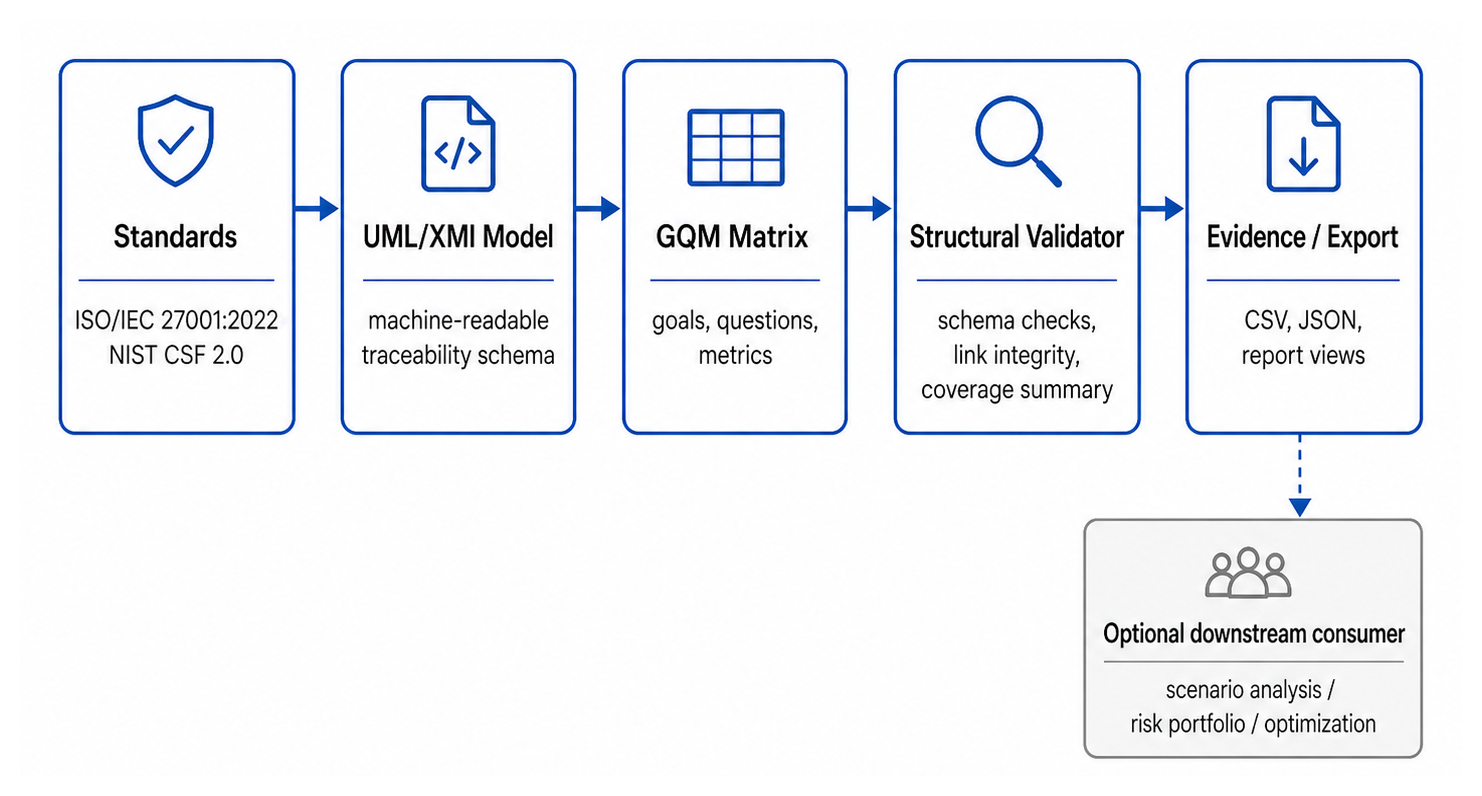
\includegraphics[width=0.96\linewidth,height=0.36\textheight,keepaspectratio]{figures/figure_1_standards_traceability_architecture.png}
\caption{Standards-to-evidence architecture from the inspected engineering artifact. This depicts a process architecture, not an observed improvement over a competing workflow.}\label{fig:arch}
\end{figure}

\begin{figure}[tbp]\centering
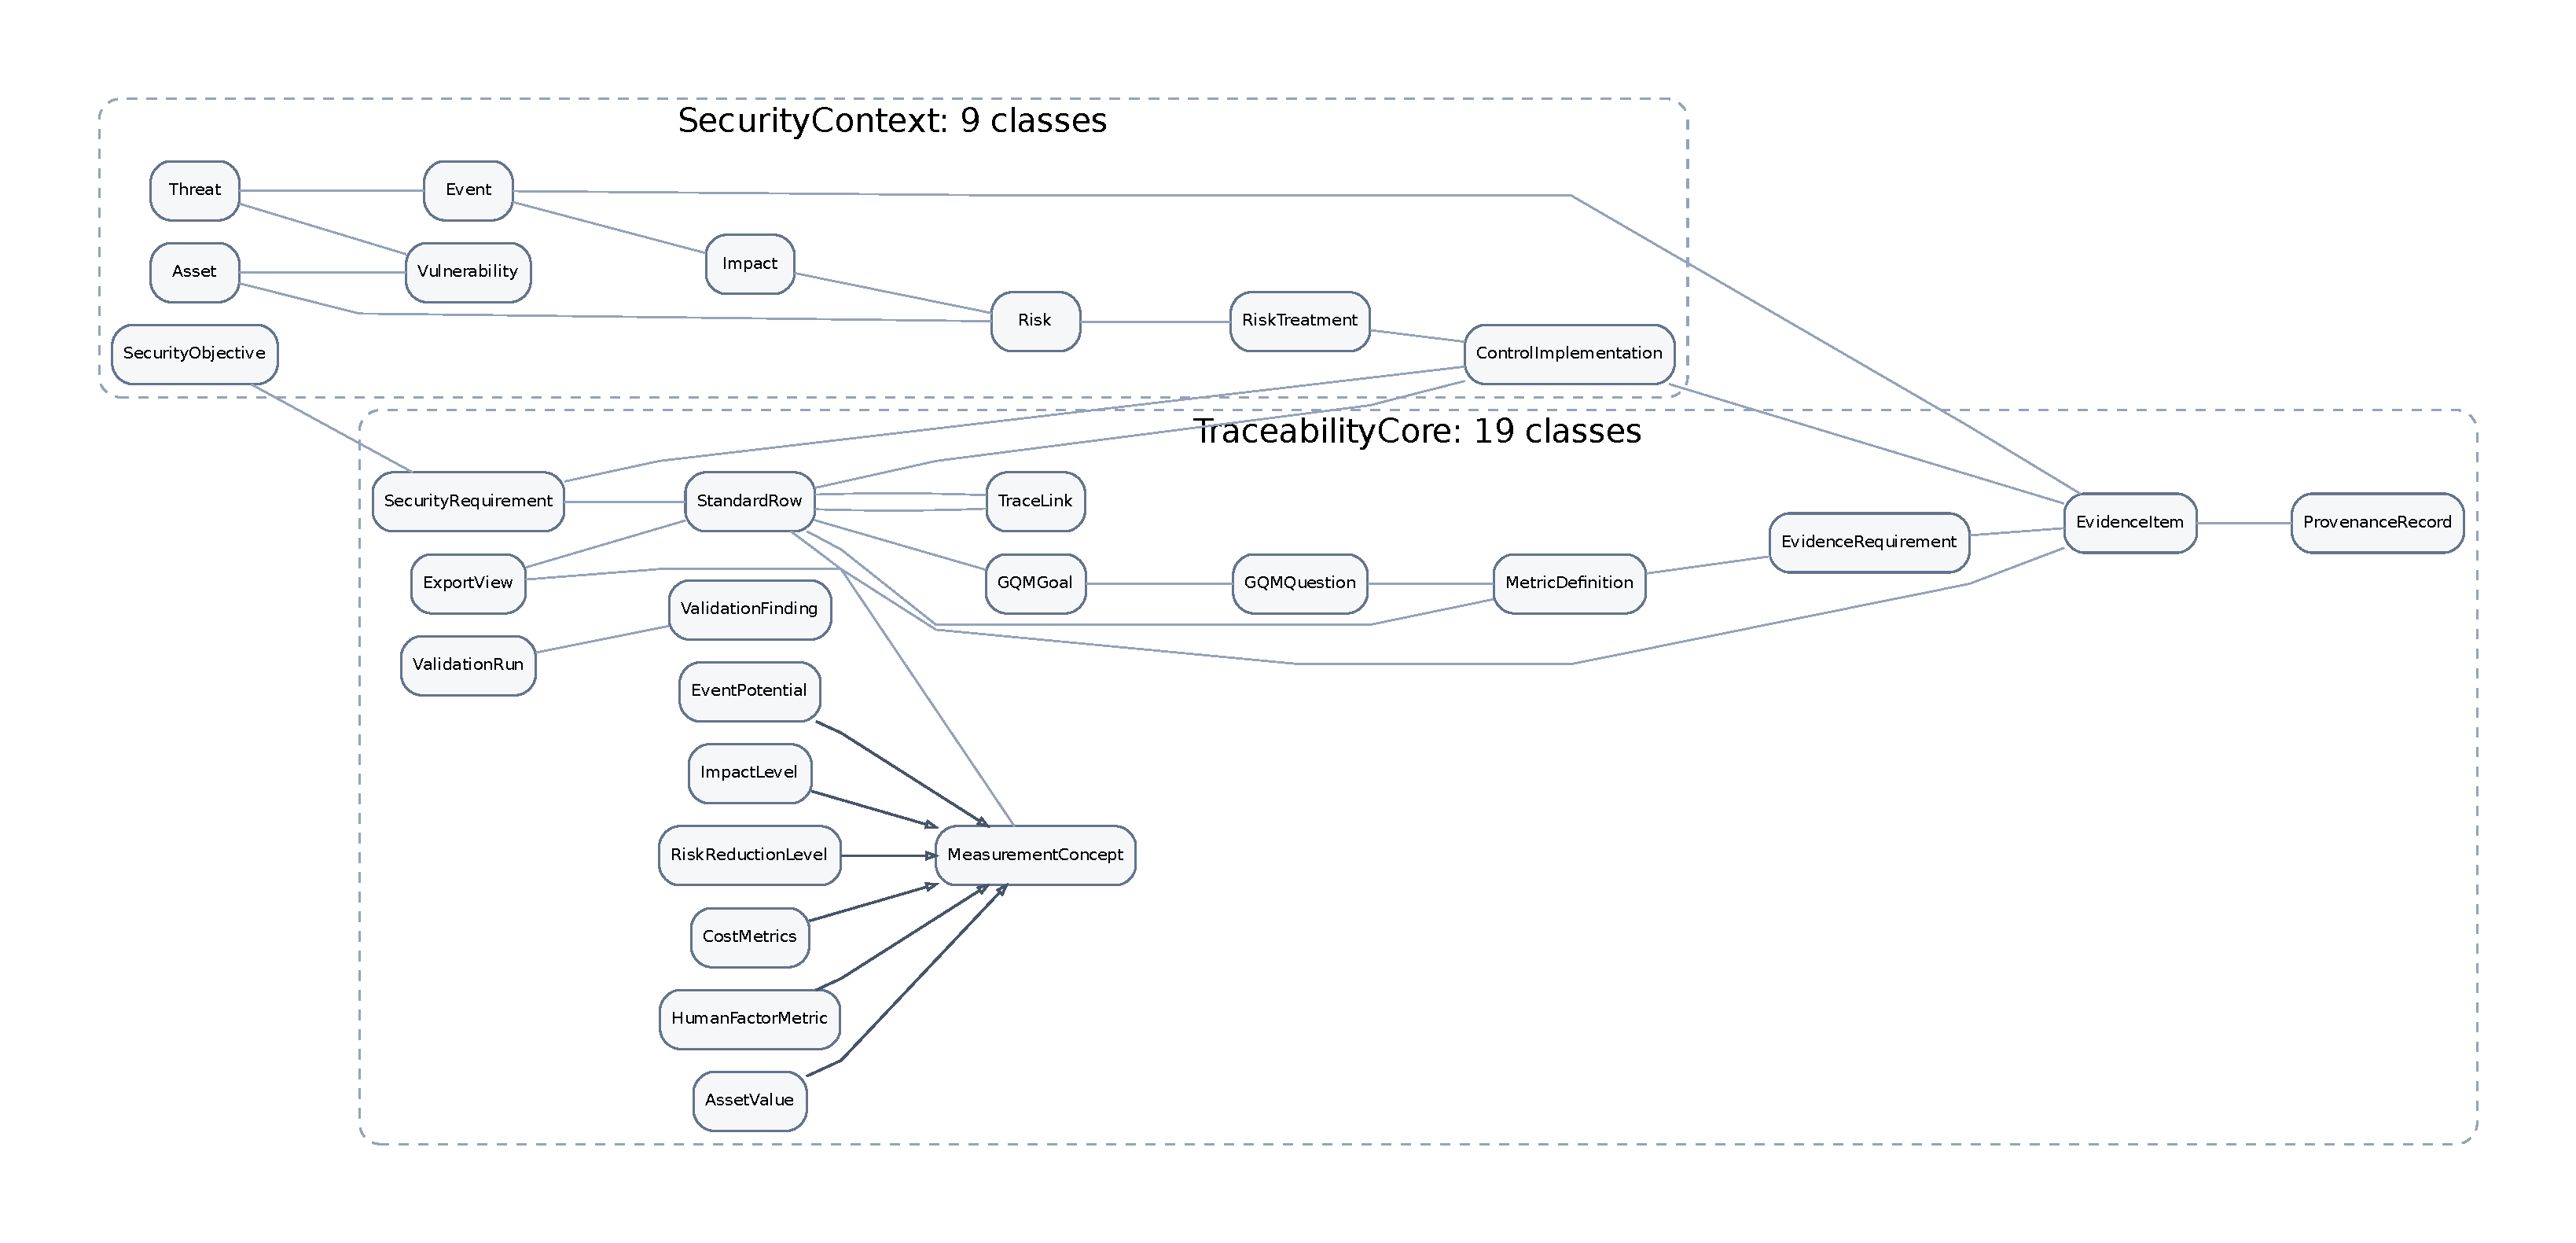
\includegraphics[width=0.99\linewidth,height=0.39\textheight,keepaspectratio]{figures/figure_stage5_canonical_full_graph.pdf}
\caption{Complete 28-class connectivity extracted directly from the canonical UML/XMI (19 TraceabilityCore and 9 SecurityContext classes, 27 binary associations shown as undirected relationships, and six inheritance arrows). The model ledger in Section~\ref{sec:uml-ledger} supplies all 28 class names, 27 association end pairs and their cardinalities; the archived technical appendix carries the complete 79 attribute specifications and seven enumerations and constraints. The A4 view suppresses small per-edge annotations; a separate, print-size A2 vector foldout is provided for readable inspection. The diagram shows a class model, not 199 populated control instances.}\label{fig:uml}
\end{figure}


\subsubsection{Source architecture and seven-column record grain}
\label{sec:overall}

The evaluated artifact organizes existing modeling, checking and export functions into a standards-to-evidence traceability pipeline (Fig.~\ref{fig:arch}). UML/XMI exchange, structural validation and report generation are supporting engineering operations, not standalone research contributions; scenario outputs are downstream illustrations.


For the source design, a \emph{standards row} is one normalized traceability record whose primary standard identifier denotes exactly one ISO/IEC~27001:2022 Annex~A control or exactly one NIST CSF~2.0 subcategory. In the historical submitted seven-column base mapping, the row stores \texttt{framework}, \texttt{id}, \texttt{title}, \texttt{metric\_ids}, \texttt{uml\_class}, \texttt{gqm\_ref}, and \texttt{linked\_ids}. Evidence-status and semantic-review status are separate enrichment fields and are not claimed to be physically present in that base CSV. Thus, the reported counts of 93 ISO rows and 106 NIST rows denote representation records, not claims that every row is evidence-populated or semantically equivalent to a row in the other standard.


\begin{table}[tbp]\centering\scriptsize
\caption{Construction rule from the seven-column baseline; provenance/enrichment is separate from the base mapping.}\label{tab:seven-col-construction}
\begin{tabularx}{\linewidth}{@{}p{0.19\linewidth}p{0.30\linewidth}Y@{}}\toprule
Source column & UML/XMI role & Interpretation / non-inference \\\midrule
\texttt{framework}, \texttt{id}, \texttt{title} & \texttt{StandardRow} identity and label & 199 standards rows, not 199 evidence instances. \\
\texttt{gqm\_ref} & \texttt{GQMGoal.goalId} & Refers to separate GQM question text. \\
\texttt{metric\_ids} & Legacy \texttt{MetricDefinition} references & Derived accepted recommendations must override obsolete legacy identifiers. \\
\texttt{uml\_class} & Historical \texttt{MeasurementConcept} anchor & Derived \texttt{proposed\_uml\_anchor} supplies the effective \texttt{EvidenceRequirement} recommendation. \\
\texttt{linked\_ids} & \texttt{TraceLink} target identifiers & Candidate cross-standard relationships; no automatic semantic equivalence. \\
\bottomrule\end{tabularx}
\end{table}

\begin{enumerate}[label=\arabic*),leftmargin=*]
  \item \textbf{Standards source layer} identifies the ISO/IEC~27001:2022 controls and NIST CSF~2.0 subcategories represented in the artifact. The layer establishes row-level identifiers and titles only; it does not imply that each row already has deployment evidence.

  \item \textbf{UML/XMI representation layer} separates a \texttt{TraceabilityCore} package (standards rows, requirements, GQM references, metrics, evidence, provenance, validation records, and exports) from a \texttt{SecurityContext} package (assets, threats, vulnerabilities, events, impacts, risks, risk treatments, security objectives, and control implementations). This preserves the security-context representation scope without conflating contextual security entities with the standards-to-evidence traceability core.

  \item \textbf{GQM/evidence-intent layer} links standards rows to goals, evidence requirements, optional quantitative questions, and provenance-bearing evidence. The adjudicated GQM catalog contains 199 evidence-first questions and 58 recorded metric-specific questions across 30 rows (257 questions in total). One metric-question link was later retired as a recommendation, leaving 57 active recommendations but retaining the 58th item as a traceable historical record. These links support representation-level traceability and reviewable mapping intent, while semantic adequacy remains bounded by the independent semantic-audit protocol described in Section~\ref{sec:semantic-audit-method}.

  \item \textbf{Structural validation layer} uses the archived canonical mapping validator to check mapping inventory and required columns, duplicate/dangling identifiers, metric-ID and \texttt{uml\_class} resolution, GQM-reference presence, normalized catalog/title contracts, duplicate link tokens, malformed-XMI handling, and reciprocal crosswalk consistency. Seven documented UML/OCL-labelled constraints are checked in separate Python OCL-equivalent fixtures; the released mapping validator does not execute a third-party OCL engine. These checks therefore establish bounded referential/structural integrity for the tested contract, not semantic correctness, general UML conformance, or auditor approval.

  \item \textbf{Evidence/export layer} registers public telemetry-derived evidence records and exports CSV, JSON, and report-oriented views with provenance tags. Representations for vulnerability intelligence, control assessments, audit records, human-factor information, and scenario assumptions remain explicitly labeled as non-instantiated when public-profile evidence is unavailable.
\end{enumerate}

Connectors and data flows in Fig.~\ref{fig:arch} denote the activated artifact path and the optional downstream-consumer boundary. This organization enables software engineers, testers, and auditors to inspect the represented evidence chain from standards rows to reporting exports, subject to the evidence-status and deployment-boundary labels stated in the artifact.
% --------------------------------------------------

\subsection{Model inventory, relational grain, and executable mapping view}
\label{sec:model-inventory}
The complete 28-class graph in Fig.~\ref{fig:uml} is derived from the unchanged canonical XMI. The subsequent vector diagram, Fig.~\ref{fig:conceptual_uml}, is deliberately a readable \emph{subset projection} of documented class names and associations; it is not presented as a second complete XMI inventory. A machine-generated inventory enumerates its 28 classes in two packages, 79 typed attributes, 27 named binary associations (54 ends, including their target types and multiplicities), six generalization links, seven enumerations, and seven named constraint bodies. The complete attribute/cardinality tables and canonical reference hash are included in Supplementary Appendix S20--S22. Crucially, these represent the \emph{class-model schema}, not 199 serialized standards instances, 212 equivalence assertions, or a new populated-XMI round trip. The archived Papyrus and Enterprise Architect observations remain specific to the earlier exports.

The coordinator-ratified derived mapping intentionally retains historical candidate columns. Across all 199 rows, \texttt{uml\_class} stores an obsolete contextual measurement-concept anchor (one of four old classes), whereas the effective \texttt{proposed\_uml\_anchor} is \texttt{EvidenceRequirement}. Similarly, \texttt{metric\_ids} records legacy proposed metrics whereas \texttt{recommended\_metric\_ids} contains the accepted direct-metric recommendations: 170 rows have no recommendation, while 29 rows carry 57 recommended metric-question links. The historical 58-question file spans 30 rows and retains the retired record. A separate, reproducible \emph{materialized effective view} was generated mapping the latter fields to explicitly named effective columns, preserving original columns in parallel for audit. This is a CSV interpretation/projection, \emph{not} a modification to the frozen data or proof that 199 evidence items were collected. The old fields must not be read as the ratified operational graph.

\subsubsection{Canonical UML/XMI contract and print-readable projection}
\label{sec:arch_model}
The frozen UML~2.5.1/XMI~2.5.1 schema has 28 classes, 79 attributes, seven enumerations, 27 associations, six generalizations and seven recorded constraints. Table~\ref{tab:metamodel-contract} identifies the principal traceability entities and their source limits; Fig.~\ref{fig:conceptual_uml} is a readable vector \emph{subset} of the complete 28-class graph (Fig.~\ref{fig:uml}). Mapping pairs are row-level data, not additional class instances. The 211-pair software baseline and later derived datasets share the same schema without implying identical data states~\cite{OMG_UML_251,OMG_XMI_251,Eclipse_UML2_50_XMI}.

\begin{table}[!htbp]
\centering
\caption{Key elements of the corrected authoritative UML/XMI contract. Figure views are projections; the XMI is authoritative.}
\label{tab:metamodel-contract}
\scriptsize
\setlength{\tabcolsep}{3pt}
\begin{tabularx}{\linewidth}{@{}>{\raggedright\arraybackslash}p{0.23\linewidth}>{\raggedright\arraybackslash}p{0.27\linewidth}Y@{}}
\toprule
\textbf{Element} & \textbf{Role} & \textbf{Key constraint / source boundary}\\
\midrule
\texttt{StandardRow} & Normalized standard entry & Unique family+ID; 1 goal ID; 1..* base-row metric links; 1 row-level measurement concept; status fields optional enrichment\\
\texttt{SecurityContext} classes & security-context entities present in the historical model & Optional representation links for assets, threats, vulnerabilities, events, impacts, risks, treatments, objectives, and control implementations\\
\texttt{GQMGoal} / \texttt{GQMQuestion} & Evidence/measurement goal and question & Goal ID comes from \texttt{gqm\_ref}; The final historical catalog contains 199 goals, 199 evidence-first questions and 58 recorded metric-specific questions (57 active recommendations after the subsequent decision)\\
\texttt{MetricDefinition} & Metric semantics & Metric IDs come directly from \texttt{metric\_ids}; metrics are not subclasses of contextual measurement concepts\\
\texttt{MeasurementConcept} & Row-level conceptual binding & Abstract parent of the six submitted \texttt{uml\_class} values; linked directly from \texttt{StandardRow}\\
\texttt{EvidenceRequirement} / \texttt{EvidenceItem} & Expected / instantiated evidence & Source reference is required only for active telemetry-linked or externally supplied evidence; placeholder/extension states may omit it\\
\texttt{ProvenanceRecord} & Origin metadata & Each instantiated evidence item retains one provenance record\\
\texttt{TraceLink} & Directed cross-standard relation & Exactly 1 source and 1 target row; explicit relation type; confidence in [0,1] when present\\
\texttt{ValidationRun} / \texttt{ValidationFinding} & Validator execution / finding & Records validator outcomes; does not imply that UML multiplicity/OCL constraints are executed by the current Python validator\\
\texttt{ExportView} & Versionable export & 0..* standards rows and evidence items; generation time explicit\\
\bottomrule
\end{tabularx}
\end{table}

\begin{figure}[H]
  \centering
  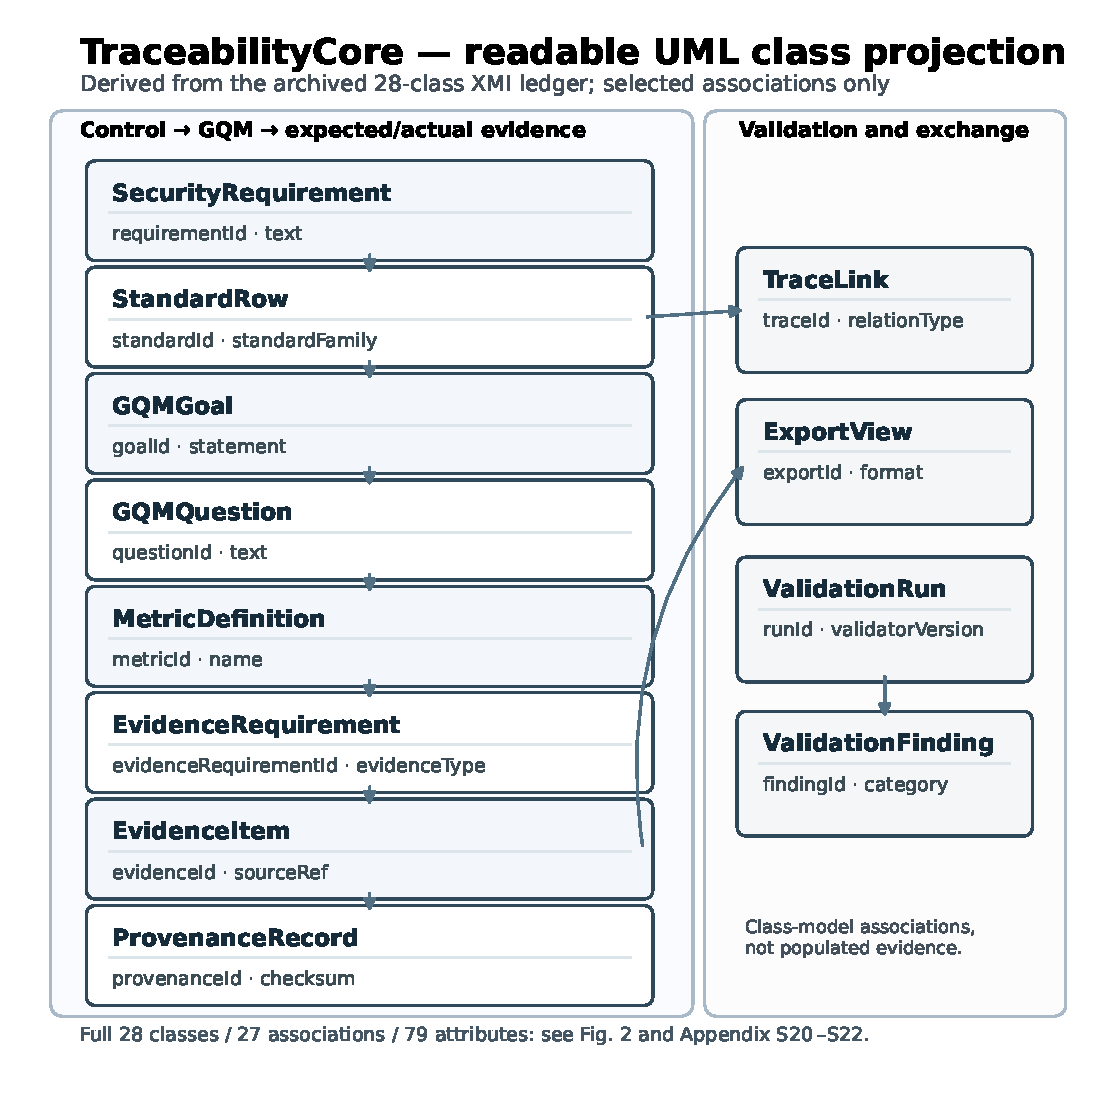
\includegraphics[width=0.96\linewidth,height=0.71\textheight,keepaspectratio]{figures/figure_2_readable_core_projection.pdf}
  \caption{Readable vector projection of selected \texttt{TraceabilityCore} classes and documented associations. \texttt{SecurityContext} is enumerated in Table~\ref{tab:metamodel-contract}; the complete 28-class/27-association XMI graph is Fig.~\ref{fig:uml} and the detailed machine-extracted ledger is in Appendix~\ref{sec:uml-ledger}. Lines indicate schema relationships, not instantiated compliance evidence.}
  \label{fig:conceptual_uml}
\end{figure}

The source-to-class identifier rules, complete attribute inventory, interchange-normalization details and historical figure projections remain in the versioned technical source and long-form record; they are not independently claimed innovations.

\subsection{Evidence question construction and evaluative units}
The originally frozen 199 source questions collapse to one normalized template after removing identifiers and titles. The 17-evidence-kind author candidates add concrete record types and provenance fields, but some require material belonging to adjacent controls. The retrospectively documented repair procedure is: (i) retain the frozen control ID, source and v1 question; (ii) record the scorer-labelled unsupported-prescription flag and its neighbouring-control rationale; (iii) replace the broad evidence-kind list with records justified by the \emph{stated} control outcome, retaining source, owner, date and evidence gaps; and (iv) preserve both wordings and compare v1--v2 under the same scoring rubric. These are manually authored and judged repairs, \emph{not} automated normative entailment checks. For example, the v1 \texttt{A.6.1} screening question also solicited unrelated employment and non-disclosure records; its v2 wording restricts examples to screening evidence. The evaluation has three distinct layers rather than one pooled test.

\textbf{Primary controlled-question assessment:} The fixed comparison contains 24 tasks (12 ISO and 12 NIST); each task includes its frozen source question and an author candidate. Two scorer-labelled workbooks each record 48 question presentations, producing 96 entries. The primary independent unit for paired analysis is the \emph{control/task}, not each recorded score. \textbf{Exploratory coverage assessment:} Four additional, purposively chosen controls covered four evidence-kind categories missing from the primary selection; the two scorer-labelled workbooks contain 16 more presentations. These four are analyzed separately, because their selection followed identification of coverage gaps. \textbf{Targeted remediation follow-up:} Fifteen unique controls carrying earlier unjustified-prescription flags were revised to author-defined, control-scoped v2 questions. The same two scorer-labelled workbooks each record 15 v1 and 15 v2 questions (60 presentations overall). The v2 revision explicitly avoids treating neighboring requirements as mandatory for the assessed control. Its primary estimand is the paired within-control difference between v1 and v2 for \emph{previously flagged cases}, not an unbiased population-level treatment effect.

All scored forms provide a 1--5 scale for semantic fidelity, evidence actionability and provenance verifiability; the unsupported-prescription flag is Y/N. The analysis calculates arithmetic means of the observed ratings, paired within-control differences, and descriptive task-level percentile bootstrap intervals. The primary evaluation uses 10,000 task resamples; the targeted follow-up similarly reports the descriptive intervals in its frozen validation output. The analysis does not use scorer-presentations as independent experimental units or re-label exploratory outcomes as confirmatory evidence. The fixed 24-task registration timestamp was not independently verified. An R015 design/status snapshot records the four-task add-on as not collected with zero scored responses, while later R016/R017 evidence includes scored four-task workbooks; the archive does not independently authenticate this chronology. The later worksheets are treated here as coordinator-attested recorded values, not verified expert approval. Existing coordinator/author statements about evaluator identity, independent delivery, source access and consent are not independently authenticated; this reanalysis verifies file hashes and arithmetic only, not identity, expertise, independence, consent or ethics authorization.

The archived forms omit condition identity, and presentation order differs between scorer-labelled workbooks; wording style nevertheless exposes the condition to a simple lexical rule. Accordingly, the study is \emph{condition-label masked, not linguistically blinded or double blind}. The archive does not establish whether the same people produced these records or what prior exposure they had, so no person-level blinding or memory claim is made.


\subsection{Human assessment streams, competence records, and evidence status}
\label{sec:humanprovenance}
Three distinct samples must not be conflated. First, a historical independent standards-row semantic classification assessed \emph{60 of the 199 mapping rows} (30 ISO/IEC 27001 and 30 NIST CSF entries) and reached 47 accept and 13 minor-revision decisions after adjudication. Initial overall decisions differed on five rows (55/60 agreement, reported unweighted Cohen's $\kappa=0.762$)\footnote{The historical dimension-level table separately reports UML-fit agreement of 56/60 ($93.33\%$) with $\kappa=0.000$. Reviewer B used only the ``yes'' category; this single-category marginal makes $\kappa$ degenerate and non-interpretable as a chance-corrected reliability estimate. The raw agreement is descriptive only and does not establish independent assessor reliability.}; six distinct rows exhibited a disagreement in at least one assessed dimension. This older sample tested the \emph{mapping-level semantic fit}, not comparative actionability of the later evidence-question variants. Second, the primary and exploratory question assessments evaluated \emph{28 distinct controls} (24 primary and four purposive exploratory tasks); they assessed formulations, not 28 additional standards-row mapping cases. Third, the targeted recheck contains \emph{15 previously flagged controls drawn from the same 28}, not 15 newly recruited controls; 12 arose from the primary cohort and three from the exploratory add-on. Consequently, the unique control population for the new question-comparison claim is 28/199, whereas mapping-level judgments have a separate 60/199 denominator. The exact identifier overlap is 11 controls between the historical 60 mapping-row sample and the newer 28-question sample, including five of the 15 targeted repairs; these overlaps do not make the separate assessment constructs interchangeable. The overlap ledger documents these relationships without presenting a combined certified-count numerator. A separate full-catalog machine audit confirmed 199 unique row keys, 199 aligned evidence-first questions, and 422 reciprocal directed references (211 undirected pairs) without dangling targets in the frozen baseline. The 139 historically unassessed rows (63 ISO, 76 NIST) were subsequently evaluated in two assessor-labelled records, yielding 114 accept and 25 minor-revision consensus entries; these complement the earlier 47/13 historical decisions. The sign-off and nine disagreement decisions are recorded, but independent confirmation of the assessors' identities and direct signatures is not part of the available audit trail. The review records are therefore not interchangeable with independently authenticated practitioner evaluations or the distinct 28-control question experiment.

The two score streams are labelled R1 and R2 in public study tables; the persons behind those labels are not independently authenticated. The newly supplied private individual PDF statements include named persons, affiliations, experience assertions, claimed standard editions, independence and conflict-of-interest declarations and sign-off codes; their SHA-256 values are independently reproducible. However, their contents remain \emph{self-declarations} until a trustworthy institutional source directly confirms signer identity, employment/qualifications, authorship and consent. Visual inspection found printed ``Signed'' labels, not handwritten marks, and automated PDF inspection found no embedded signature fields. No independent verification of standard licensing, ethics/exemption decisions or calibration was supplied with the byte-level archive. Thus, prior rating summaries and these new documentary statements remain distinct from authenticated independent practitioner assessments. Personal identifiers and PDF copies are stored only in a restricted evidence location and should not be released in a public supplement.

\subsubsection{Semantic-review protocol and limits}
\label{sec:semantic-audit-method}
Structural identifier coverage and expert semantic agreement are distinct evidence types. The historical review concerned 60 of 199 standard rows (30 ISO, 30 NIST), followed by a separate first-pass A/B-labelled review of the remaining 139 rows; recorded final outcomes sum to 161 accepted and 38 minor-revision decisions. In the 139-row cohort, decisions agreed on 130/139 records ($93.53\%$, Cohen's unweighted $\kappa=0.784$), with nine documented adjudications. Reviewers' names and credentials in the supplied PDFs have not been independently authenticated. Source editions and external NIST OLIR references are treated as comparison aids rather than conclusive semantic ground truth~\cite{NIST_OLIR_218,NIST_OLIR_FAQ}. The complete sampling, rubric, disagreement ledger and fresh-sample composition are preserved in the archived audit package, not pooled with the separately selected 15-question repair evaluation.

\subsection{Crosswalk decisions and informative-reference comparison}
The accepted extended catalog is a derived copy; the 211-pair frozen original remains unchanged. The coordinator-accepted changes removed the link \texttt{ID.RA-03}--\texttt{A.8.16}, added \texttt{PR.PS-03}--\texttt{A.7.14}, and added \texttt{ID.IM-03}--\texttt{A.5.36} while preserving the already recorded partial \texttt{A.5.27} link. ISO 27001 clauses 10.1/10.2 are \emph{not} introduced as Annex A rows. The resulting 212 undirected reciprocal relations comprise 424 directed link entries; this projection is not itself a populated UML/XMI instance experiment.

For descriptive contrast, the same pinned NIST OLIR Reference 218 workbook (version 1.0.0, posted 2026-07-09; raw SHA-256 \texttt{7ba6a8c3\allowbreak fa5207f8\allowbreak 4b1a7248\allowbreak 0fa5bfac\allowbreak c6326ab9\allowbreak 7bf6e28a\allowbreak ab631bd3\allowbreak cf626848}) was compared with all three mapping states~\cite{NIST_OLIR_218}. Exact-pair overlap/union and Jaccard were 38/266 and 0.1429 for the frozen 211-pair baseline, 38/267 and 0.1423 for the distinct 212-pair projection, and 40/245 and 0.1633 for the 192-pair 192-pair candidate. ISO-control/NIST-subcategory coverage was respectively 68/93 and 89/106, 69/93 and 89/106, and 71/93 and 86/106; counts of ISO controls with multiple NIST links and NIST subcategories with multiple ISO links were 46/43, 47/43, and 43/40. The comparator has no populated relationship-strength cells, so primary/secondary, equivalence, or ambiguous labels are unavailable. These structural differences do not establish semantic correctness, and OLIR is not treated as ground truth. The pinned workbook's raw SHA3-256 differs from the checksum recorded in the catalog; this remains a provenance limitation, not evidence of tampering.


\subsubsection{Validator implementation and archival robustness protocol}
\label{sec:validator}
The Python validator checks the required seven-column row inventory, unique standard IDs, metric and GQM references, UML class-name resolution, linked standards identifiers and reciprocal crosswalk consistency. It emits structured findings but does \emph{not} execute the documented UML multiplicity or OCL constraints, adjudicate normative equivalence, or establish organizational evidence sufficiency. A local archived archived structural report records an earlier synthetic evaluation with 40 valid perturbations, 55 deliberately malformed/incorrect artifacts over 11 defect families, and 20 mixed artifacts. The exact case inputs and generator for these 40/55/20 cases were not recovered in the accessible evidence package; these counts are therefore historical reported values, not results independently reproduced in this revision. The units and original-versus-extended checker are not equivalent to field audit outcomes; the reported quantitative results are in Section~\ref{sec:structural-results}.

The frozen 199-row catalog has 199 goal IDs, 199 evidence-first questions and 58 historical metric-specific questions (257 in total). The later derived mapping retains 57 active metric-question recommendations and one retired historical record; supported evidence types and the selected GQM question-repair study are assessed separately. Repository source modules expose the checker's CLI, ingestion, optional telemetry producer and reporting outputs (\RepoLink); no organization-specific asset valuation, CVSS asset linkage, human-factor record or measured intervention effect was instantiated. The accessible technical archive retains aggregate reports and selected earlier source/test artifacts, but not the exact 40/55/20 case corpus and its generator.

\subsection{Trace walkthrough: A.5.1 from catalog row to evidence intent}
\label{sec:trace-example}
A concrete reconstructed trace tests whether data identifiers and question text can be followed across the frozen files without fabricating an organizational assessment. The accepted derived ISO/IEC~27001 Annex A row \texttt{A.5.1} (\emph{Policies for Information Security}) has \texttt{gqm\_ref=GQM-ISO-001}; the archival GQM catalog resolves it to \texttt{GQM-ISO-001-EVID-01}, a provenance-oriented evidence question; its \texttt{evidence\_kind} is \texttt{PolicyProcedureEvidence}. The effective UML class anchor is \texttt{EvidenceRequirement}, and \emph{no direct metric is currently recommended}. The older \texttt{HumanFactorMetric} class and \texttt{HF\_AWARENESS;TCO\_3Y} fields are retained only as source-history fields, not silently used as current anchor or metrics. Three NIST links are present and reciprocal: \texttt{GV.OV-03}, \texttt{GV.PO-01}, and \texttt{GV.PO-02}. The complete exact-text question and machine-readable link verification are provided in Supplementary Appendix S23 and the \texttt{WORKED\_TRACE\_A5\_1} JSON file.

This walkthrough has \textbf{zero observed organizational EvidenceItem records}: no policy document, owner signature, validity period, auditor decision, or actual provenance URI is inferred. The model can specify the required evidence class and linking intent, but no control-compliance or evidence-completeness finding follows. Validation of 199 reciprocal row references establishes structural consistency, not semantic equivalence between a given ISO control and NIST subcategory.

\subsubsection{Trace-to-export transformation and bounded evidence consumers}
\label{sec:math_human}

\begin{table}[H]
\centering
\caption{Activation boundary in the strict public-data profile.}
\label{tab:risk_factor_activation}
\small
\setlength{\tabcolsep}{4pt}
\begin{tabularx}{\textwidth}{@{}p{0.22\textwidth}p{0.33\textwidth}X@{}}
\toprule
Component & Public-profile status & Evidence interpretation \\
\midrule
Telemetry score & Activated through calibrated IoT flow scores & Demonstrates evidence generation and provenance capture. \\
Asset value & Source-cohort telemetry proxy & Represents the field; does not validate enterprise asset valuation. \\
CVSS prior & Global neutral prior & Represents a non-instantiated CVSS field; row-varying CVE effects are not validated. \\
Human factor & \texttt{HF:none} & Represents the slot; does not validate organizational HF effects. \\
Device/time & Source-file cohorts and synthesized ordering & Supports boundary-safe public evaluation; not true device-level chronology. \\
Control catalog & Configurable catalog assumptions & Supports scenario exploration only; not measured intervention effectiveness. \\
\bottomrule
\end{tabularx}
\end{table}

This layer converts represented evidence into exportable records while preserving provenance. The public profile activates only the telemetry-derived evidence path. Other fields--asset value, CVSS exploitability, human-factor information, and control effectiveness--are retained as typed extension points and are explicitly tagged as proxies, neutral priors, inactive overlays, or scenario assumptions. Table~\ref{tab:risk_factor_activation} centralizes the public-profile evidence scope so that the reported experiment is not misread as a full empirical validation of a risk-scoring engine.

Figure~\ref{fig:conceptual_uml} gives the compact traceability view for this evidence interface. Standards rows are connected to GQM goals, questions, metrics, evidence items, and export views; the structural validator checks schema and link integrity; optional downstream consumers can read exported records for reporting or scenario analysis without becoming part of the primary claim.


% --------------------------------------------------

\subsection{Typed interchange and software tests}
An archived two-tool experiment imported, edited and exported the canonical model using Papyrus 2025-06 (Eclipse 4.36) and Enterprise Architect 17.2.1721. A typed comparator normalizes permitted tool-generated identifiers/wrappers and checks named class/package inventories, property type and bounds, association endpoints, generalization endpoints, enumeration literals, and seven stored constraint bodies. The comparison reanalyzes \emph{real historical tool exports}; it is not presented as a new GUI rerun, general UML semantic equivalence or runtime OCL evaluation.

A separate Python mapping validator checks identifiers, schema-field completeness, model classes, metrics, cross-standard endpoints, selected multiplicity contracts and structurally detectable reference faults. The current canonical regression suite checks the XMI~2.5.1 inventory (28 classes, 79 attributes, 27 associations/54 ends, six generalizations and seven stored constraints) and injects a wrong association target type to verify structured rejection. These are structural checks; they do not execute the seven OCL bodies. The archived archived structural report records 40 valid boundary artifacts, 55 held-out defect artifacts, and 20 mixed-fault artifacts, but the exact corpus and generator were unavailable for replay in this revision. A smaller distinct comparator reports 15 deliberately selected negative cases plus two valid cases; the old/reference checker and typed checker have unequal implemented scopes. All historical counts measure sensitivity on authored fixtures, not generalized superiority across other requirements-engineering methods.


\subsection{Public CICIoT2023 evidence interface and reproducibility boundary}
\label{sec:telemetry-method}
The archived public CIC~IoT~2023 profile~\cite{Neto2023_CICIoT2023,CICIoT2023_Web} uses the merged CSV release as an \emph{evidence-signal generator}, not as ground truth for the 199 standards mappings or for human GQM ratings. The recorded \texttt{real} profile reads 63 source CSV files with a cap of 1,000 rows per file (63,000 raw rows), derives surrogate cohorts from source-file identifiers where actual device identifiers are unavailable, and constructs ordered train/validation/test windows. When capture timestamps are absent, \texttt{data\_ingest.py} synthesizes ordering indices beginning on \texttt{2025-01-01}; such values do not denote observed capture times or a prospective temporal holdout. The original 63 input files and per-file checksums are not contained in the available research package, so a new end-to-end training rerun cannot be claimed. The historical test partition contains 8,784 windows, of which 226 are benign. All aggregate counts below refer to the archived outputs and were reaggregated without refitting a model.

The recorded fixed-FPR operating point was selected from \emph{pre-test out-of-fold} reference scores with a target reference FPR $\leq0.05$: the selected threshold is 0.86087, reference FPR 0.03979, and reference detection rate 0.98513. That threshold was applied unchanged to the held-out partition; the test FPR and recall are Results rather than criteria used to tune the test threshold (Table~\ref{tab:stage6_confusion}). This evaluation measures an evidence-reporting diagnostic under an attack-dominant sample, not real-device transfer, deployed IDS performance or organizational control compliance.

\subsubsection{Telemetry feature and provenance interface specification}
\label{sec:dataset}
\label{sec:model-details}
The software interface is classifier-agnostic: a compatible scorer exports a surrogate cohort/source identifier, ordering index or observed timestamp when available, calibrated suspiciousness score, selected operating threshold, optional alert label, and record/configuration provenance. The archived default implementation combines an LSTM-style anomaly score with gradient-boosted probabilities; this study does not demonstrate classifier superiority. Asset-value, row-level CVE/CVSS exploitability, human-factor observations and measured intervention effects are not usable original CICIoT features in this profile. The CVSS path applies a global neutral prior, human-factor provenance is marked \texttt{HF:none}, and asset value is a telemetry-derived proxy rather than a verified enterprise asset appraisal. These fields are model extension points and are not silently used as measured inputs to the classifier.

Generated evidence summaries and metric definitions are linked to the GQM/standards view and exported as validation reports, evidence records and reporting-oriented CSV/plot outputs. Neither the exported artifacts nor the optional scenario consumer constitutes an independent control-compliance assessment. Configuration details and supplementary numerical outputs remain versioned separately from this method description.

\section{Results}\label{sec:results}
\noindent\textbf{Result provenance.} Archived software-test outputs and tool exports are treated as historical observations. Human question ratings and the ratified 212-pair mapping are subsequent, distinct analyses. The available source logs were re-aggregated; model training and end-to-end graphical interchange steps were not repeated.

\begin{table}[tbp]\centering\footnotesize
\caption{Methods-to-results alignment. Each row has a distinct unit and a different inference boundary; counts must not be pooled.}\label{tab:results-route}
\begin{tabularx}{\linewidth}{@{}p{0.18\linewidth}p{0.22\linewidth}Y@{}}\toprule
Claim / check & Measured unit & Where the result and boundary are reported \\\midrule
Primary RQ & Fixed 24-task wording comparison; four exploratory tasks separate & Generic vs specific question ratings, overreach flags and selected 15-control repair; no population-level or causal inference. \\
EC1 & XMI and tool-export fields & Version-bounded Papyrus/EA preservation; not general interoperability. \\
EC2 & Mapping rows and undirected pairs & Historical 211, derived 212 and later 192-pair recorded states are version-separated; structural agreement is not semantic certification. \\
EC3 & Authored faults, five constructed traces, archived telemetry windows & Fixture-level detection and source-audited telemetry; neither field lifecycle performance nor device-level generalization. \\
\bottomrule\end{tabularx}
\end{table}

\subsection{Primary and exploratory question comparisons (RQ)}
\begin{table}[tbp]\centering\small
\caption{Source-recomputed primary and separately analyzed exploratory question-score records (five-point scores). Scorer-presentations are \emph{not} independent inferential units; external score-source authentication remains open.}\label{tab:expert}
\begin{tabular}{@{}p{4.2cm}rrrr@{}}\toprule
& Source & Candidate & Paired delta & Overreach \\\midrule
Primary, 24 tasks: actionability & 2.00 & 4.17 & +2.17 & 23/48 \\
Primary: semantic fidelity & 3.94 & 3.63 & $-0.31$ & --- \\
Primary: provenance & 2.00 & 5.00 & +3.00 & --- \\
Exploratory, 4 tasks: actionability & 2.00 & 4.25 & +2.25 & 6/8 \\
Exploratory: semantic fidelity & 4.00 & 3.50 & $-0.50$ & --- \\
Exploratory: provenance & 2.00 & 5.00 & +3.00 & --- \\
\bottomrule\end{tabular}\end{table}

On the fixed 24 tasks, the actionability mean difference was +2.1667 with descriptive task-bootstrap 95\% percentile interval [+1.8333,+2.4583]. It was positive on 23 tasks, tied on one and negative on none; a two-sided exact sign test gives $p=2.38\times10^{-7}$ under independent task-pair and symmetric-null assumptions. Semantic fidelity changed by $-0.3125$ (interval [$-0.6667$,+0.0833]); it decreased on 14 tasks, tied on four and increased on six (exact sign-test sensitivity $p=0.115$). Provenance increased by +3.00. These task-level tests are conditional sensitivity summaries, not confirmatory population inference: the tasks are fixed, no independently timestamped registration was verified, and the task set is not a probability sample. The initial specific wording incurred 23 overreach flags across 48 candidate presentations, involving 12 controls. The separate, purposively selected four-task missing-kind add-on had six flags across eight candidate presentations involving three additional controls; its 16 recorded presentations are not pooled with the primary 96. The 24- and four-task workbooks reconcile to the preserved task-level summaries, but an earlier study-status snapshot says the add-on was not collected while later available records contain scored sheets; chronology, scorer identity and expert status are not independently authenticated. Across these separate cohorts the recorded flags concern 15 distinct controls, \emph{not} a 15/199 random sample. Exact agreement between the assessor A/B-labelled streams on primary fidelity was 45/48 and on actionability 48/48; agreement does not eliminate shared framing or expectancy risk.

\subsection{Targeted question repair follow-up (RQ)}
The targeted follow-up comprises records for fifteen previously flagged controls, two conditions, two scorer-labelled workbooks and 60 complete presentations (30 per condition; no recorded abstentions or missing values). The workbooks carry coordinator/participant references, but institutional ethics authorization, consent, scorer identity, qualifications and independence are not independently authenticated; no ethics approval or expert certification is inferred. Only privacy- and license-cleared aggregates are candidates for release; the source workbooks and question prose remain restricted.

\begin{table}[H]\centering\small
\caption{Targeted control-question follow-up. Each condition has 30 scorer-presentations over 15 paired controls. Descriptive intervals resample controls, not the 30 records as independent participants.}\label{tab:r018}
\begin{tabular}{@{}lrrr@{}}\toprule
Outcome & Candidate v1 & Control-scoped v2 & Paired delta \\\midrule
Semantic fidelity (1--5) & 2.9667 & 4.8667 & +1.9000 \\
Evidence actionability (1--5) & 3.6667 & 4.7667 & +1.1000 \\
Provenance verifiability (1--5) & 5.0000 & 4.9333 & $-0.0667$ \\
Unjustified-prescription flags & 29/30 & 0/30 & --- \\
Joint quality pass (post hoc) & 1/30 & 30/30 & +29/30 \\
\bottomrule\end{tabular}\end{table}

The additional \emph{post-hoc} joint pass requires fidelity, actionability and provenance each at least 4/5, with no unsupported-prescription flag. Recalculation from both frozen rating workbooks gives 1/30 for v1 and 30/30 for v2 (15 controls, two scorer labels); all 15 controls pass under both labels only after repair. A descriptive 10,000-resample control-level bootstrap of the paired pass difference (+29/30) yields [0.90,1.00]. This is an exploratory composite, not a pre-registered independent endpoint, a general success probability or a superiority estimate versus OSCAL. The corresponding descriptive task-bootstrap intervals remain [+1.7667,+2.0333] for fidelity and [+0.8000,+1.4333] for actionability. Agreement between scorer-labelled streams and exposure, targeted sample selection and lack of externally verified assessor credentials preclude population, causal or expert-certification inferences. The other 171 candidate controls were not question-rated. As a threshold-sensitivity check of the same frozen ratings, requiring fidelity $\geq5$ gives 0/30 v1 versus 26/30 v2 passes; requiring actionability $\geq5$ gives 0/30 versus 23/30; requiring all three scores $\geq5$ with no over-prescription gives 0/30 versus 20/30. At the paired-control level, fidelity improves in all 15 controls, actionability in 14 (one tie), whereas provenance decreases in two; thus the contrasts are not uniform inflation of every rating dimension. These are post-hoc descriptive checks on the same selected cases, not an independent replication.


\subsection{Historical semantic repairs and follow-on approval trace}
\label{sec:repairtrace}
The historical standards-row semantic assessment is a distinct validation layer. In the first-pass overall decision, assessors A and B agreed on 55 of 60 rows; five rows differed in the overall classification, while six \emph{distinct rows} had at least one disagreement across rating dimensions. Post-adjudication classifications were 47 acceptable and 13 minor-revision. A separate seven-case reciprocal-pair consensus log records two retained links, four removed links, and one added link. These seven are \emph{pair decisions}, not seven additional rated controls. The historical post-review 211-pair crosswalk and 257-question catalog were frozen after those actions.

In the subsequent decision audit, each assessor evaluated 20 decisions: 13 wording/semantic-row repair cases plus the seven reciprocal pair decisions. Each evaluator recorded 17 \texttt{ACCEPT} and three \texttt{REVISE} outcomes, with identical revise identifiers \texttt{ID.RA-03}, \texttt{PR.PS-03}, and \texttt{ID.IM-03}. Following separate coordinator approval, these three revision requests were resolved as follows: remove the secondary reciprocal \texttt{ID.RA-03--A.8.16} link and retire the unsupported \texttt{EP\_EXPLOIT} recommendation without silently substituting a new metric; add the reciprocal \texttt{PR.PS-03--A.7.14} relation; and add a limited supporting \texttt{ID.IM-03--A.5.36} relation while preserving the explicitly partial \texttt{A.5.27} relation. Eight data-field edits across six row IDs implement these three semantic decisions, yielding a distinct 212-pair derived release; the historical 211-pair software version remains unchanged. These are documented decisions and mechanically checked table changes, \emph{not} independent full-population certification of cross-framework normative equivalence. The original 13-case repairs and seven-pair records remain individually traceable in the Supplementary decision ledger.

\subsection{Model and interchange observations (EC1)}
The checked canonical class model has 28 named classes, 79 attributes, seven enumerations, 27 associations, six generalizations and seven OCL constraint bodies. In the archived exports, normalized Papyrus preserved 7/7 checked bodies whereas Enterprise Architect preserved 0/7. The latter is a documented information-loss finding, not a PASS for constraint portability. A typed checker exposes wrong association targets even when overall element counts are unchanged; the older count-preserving check did not detect that deliberate mutation. Twelve typed comparator tests passed in the archived re-analysis. Neither result establishes preservation of populated control/evidence instances or semantics of OCL evaluation.

\subsection{Ratified mapping and OLIR contrast (EC2)}
\begin{table}[tbp]\centering\small
\caption{Version-preserving mapping counts and external-source concordance. OLIR is an informative reference, not semantic ground truth.}\label{tab:olir}
\begin{tabular}{@{}lrr@{}}\toprule
Measure & Frozen historical & Accepted extension \\\midrule
Catalog control records & 199 & 199 \\
Reciprocal ISO--NIST pairs & 211 & 212 \\
Unique OLIR comparator pairs & 93 & 93 \\
Exact shared pairs & 38 & 38 \\
Study-only pairs & 173 & 174 \\
OLIR-only pairs & 55 & 55 \\
Jaccard coefficient & 0.142857 & 0.142322 \\
\bottomrule\end{tabular}\end{table}

Table~\ref{tab:olir} compares version-specific pair sets, not equivalent control coverage or normative correctness. Historical metric-question versus active-recommendation counts are defined in Table~\ref{tab:version-states}.

\subsection{Structural robustness and trace exemplars (EC3)}
The archived archived structural report records 40 structurally valid perturbations (0 false-positive findings for the full validator) and 55 held-out synthetic defects (55/55 structured detections, versus 15/55 structured detections by the narrower reference validator and five additional unhandled malformed-XMI exceptions). It also reports 20/20 case-level detections on mixed synthetic artifacts for the full checker and 14/20 for the reference comparator. The exact inputs and generator for these suites were unavailable for replay in this analysis, so the values remain historical reported results rather than newly generated evidence. In a separate selected scope test, a reference checker caught 4/15 targeted mutations while the typed checker caught 15/15; this cannot be interpreted as the advantage of GQM over OSCAL or of automated work over human auditing. Five constructed lifecycle case records link to standard identifiers and recorded evidence states; all five seeded link faults were identified and repairable within the case-checking contract. The CICIoT2023 telemetry pathway~\cite{Neto2023_CICIoT2023,CICIoT2023_Web} exemplifies evidence and provenance serialization, not operational security-control effectiveness, compliance certification or auditor productivity.


\subsubsection{Structural and interchange checks (EC1--EC3)}
\label{sec:structural-results}
The frozen 199-row catalog resolves all 93 ISO Annex A controls and 106 NIST subcategories structurally. The historical archived structural report records no false positives on 40 held-out valid cases, 55/55 structured detections by the extended checker versus 15/55 by the narrower reference checker (with five malformed-XMI exceptions), and structured outcomes for 20/20 mixed artifacts. Because the case corpus and generator were unavailable for replay, these are retained as historical reported observations rather than newly reproduced outcomes. They do not establish comprehensive semantic correctness or organizational control effectiveness.

The recorded Papyrus/Enterprise Architect round trip concerns field preservation for this particular XMI and specific tool versions, not a new import/export mechanism. The source contract's classes, associations and attributes were preserved in both checked exports, but Enterprise Architect dropped all seven examined OCL bodies, whereas Papyrus retained them after documented serialization normalization.

\begin{table}[H]
\centering
\caption{Observed preservation in the two-tool UML/XMI round-trip experiment.}
\label{tab:uml-roundtrip-results}
\small
\setlength{\tabcolsep}{4pt}
\begin{tabular}{@{}lrrr@{}}
\toprule
Component & Canonical & Papyrus & Enterprise Architect \\
\midrule
Packages & 2 & 2 & 2 \\
Primitive types & 4 & 4 & 4 \\
Enumerations & 7 & 7 & 7 \\
Classes & 28 & 28 & 28 \\
Attributes & 79 & 79 & 79 \\
Associations & 27 & 27 & 27 \\
Association ends & 54 & 54 & 54 \\
Generalizations & 6 & 6 & 6 \\
UML/OCL constraints & 7 & 7 & \textbf{0} \\
Sentinel package/class & -- & present & present \\
\bottomrule
\end{tabular}
\end{table}

Held-out mutation families, schema/XSD/graph reference-checker contrasts and synthetic scalability runtimes are reported in the archived extended technical record; no claim of general tool superiority follows.

\subsubsection{Five constructed lifecycle cases: archived records}
\label{sec:lifecycle-multicase}


The historical lifecycle analysis is evaluated through five constructed lifecycle-facing cases rather than a single mini-case. The cases cover secure authentication, continuous monitoring, incident response, physical security monitoring, and awareness/training, thereby spanning technological, organizational, physical, and people-oriented ISO/IEC~27001 domains and multiple NIST CSF~2.0 functions. Each case is resolved against the same frozen mapping/XMI vocabulary and follows the same bounded sequence: requirement $\rightarrow$ standards binding $\rightarrow$ GQM/metric definition $\rightarrow$ evidence placeholder or telemetry observation $\rightarrow$ structural check $\rightarrow$ reportable export.

Two cases can instantiate telemetry-derived observations from the public profile, whereas three deliberately terminate in extension-only evidence hooks because the public dataset contains no operational incident-response logs, physical-security evidence, or training records. This distinction is part of the evaluation: the artifact must preserve a trace without converting unavailable deployment evidence into a false populated-evidence claim.



\begingroup
\scriptsize
\setlength{\tabcolsep}{2.1pt}
\renewcommand{\arraystretch}{1.08}
\begin{longtable}{>{\raggedright\arraybackslash}p{1.7cm}>{\raggedright\arraybackslash}p{3.0cm}>{\raggedright\arraybackslash}p{2.3cm}>{\raggedright\arraybackslash}p{3.3cm}>{\raggedright\arraybackslash}p{2.5cm}}
\caption{Five-case proof-of-concept lifecycle trace exercise for the supporting lifecycle demonstration. The final column reports canonical-trace resolution / injected-defect detection / repaired-trace resolution.}
\label{tab:lifecycle-multicase}\\
\toprule
\textbf{Case} & \textbf{Requirement focus} & \textbf{Representative ISO / NIST binding} & \textbf{Evidence mode in public profile} & \textbf{Baseline / defect / repair}\\
\midrule
\endfirsthead
\toprule
\textbf{Case} & \textbf{Requirement focus} & \textbf{Representative ISO / NIST binding} & \textbf{Evidence mode in public profile} & \textbf{Baseline / defect / repair}\\
\midrule
\endhead
\bottomrule
\endlastfoot
LC-AUTH-01 & Secure authentication / anomalous access & A.8.5 / PR.AA-03 & Telemetry observation available & PASS / DETECTED / PASS\\
LC-MON-02 & Continuous monitoring / adverse events & A.8.16 / DE.CM-09 & Telemetry observation available & PASS / DETECTED / PASS\\
LC-IR-03 & Incident-response traceability & A.5.26 / RS.MA-02 & Extension-only evidence hook & PASS / DETECTED / PASS\\
LC-PHY-04 & Physical security monitoring & A.7.4 / DE.CM-02 & Extension-only evidence hook & PASS / DETECTED / PASS\\
LC-AWR-05 & Awareness and training & A.6.3 / PR.AT-01 & Extension-only evidence hook & PASS / DETECTED / PASS\\
\end{longtable}
\endgroup


\paragraph{Lifecycle-case evidence grain and negative cases}
The five cases are five \emph{author-constructed trace fixtures}, not five organizations, projects or independent industrial replications. A fixed case-ledger audit of the archived records (Table~\ref{tab:lifecycle-multicase}) finds 5/5 baseline structural trace resolutions, 5/5 detections of one deliberately injected fault per case, and 5/5 resolutions after repairs. Two of five cases (LC-AUTH-01 and LC-MON-02) permit an illustrative public-profile telemetry observation; for the other three (LC-IR-03, LC-PHY-04 and LC-AWR-05), the evidence field is an \emph{extension-only hook} with no corresponding organizational incident, physical-security or training record. Accordingly, 5/5 is a fixture-level structural result, \emph{not} 100\% evidence availability, audit acceptance, compliant controls or full-lifecycle effectiveness. The independent-organization sample is zero. This partition is machine-auditable from the archived case-table rows and the original Step~6 report; it is a retrospective consistency check and \emph{not} a newly executed case experiment.

\begin{table}[tbp]
\centering\small
\setlength{\tabcolsep}{4pt}
\renewcommand{\arraystretch}{1.1}
\begin{tabularx}{\linewidth}{>{\raggedright\arraybackslash}p{3.55cm}>{\centering\arraybackslash}p{1.3cm}X}
\toprule
\textbf{Evidence layer} & \textbf{Count} & \textbf{Not established} \\
\midrule
Constructed trace round trip & 5/5 & No organizational evidence ingestion, user-facing workflow completion or auditor acceptance. \\
Injected structural fault and repair & 5/5 each & One authored defect per case is not an unseen field-error distribution or a statistical detection-rate estimate. \\
Telemetry-available cases & 2/5 & Open-dataset signals are not independently verified deployed-control evidence. \\
Extension-only evidence hooks & 3/5 & Unpopulated incident, physical-security and training evidence must not be counted as assessed controls. \\
Independent organizational deployments & 0/5 & No basis for cross-organization transfer, productivity or compliance-effectiveness claims. \\
\bottomrule
\end{tabularx}
\caption{Retrospective lifecycle-case evidence audit. Denominators are five authored \emph{fixtures}, not an independent population sample.}
\label{tab:c5_case_evidence_grain}
\end{table}

\paragraph{Lifecycle-case interpretation and external validity}
The five cases are authored structural fixtures: five baseline traces resolve, five different injected structural defects are caught, and all five corrected traces resolve again (Table~\ref{tab:c5_case_evidence_grain}). Only two fixtures have public-profile telemetry available; the other three contain unpopulated evidence hooks. No organizational deployment, practitioner assessment, evidence-collection-time measurement, or real-world compliance outcome was observed. A future independent assessment would require multiple organizations, practitioner task assignment, time-stamped evidence packs, blinded review and prespecified error/time outcomes; that protocol has \emph{not} been executed. The case traces cannot support industrial generalization.

\subsection{CICIoT2023 evidence-signal results (historical, not rerun)}
\label{sec:telemetry-results}
The archived operating-point outcomes are reported together with their source-exact confusion counts in Table~\ref{tab:stage6_confusion}. Classifier ranking and threshold-independent AUROC do not change when only the alert threshold changes; neither point demonstrates production deployment quality.

\subsection{Recovered historical CICIoT2023 run inputs and source-grounded outcome audit}
\label{sec:source-run-audit}
The historical \texttt{real} output directory, now associated with the pinned public software study, contains an \texttt{input\_data\_summary.csv}, \texttt{split\_summary.csv}, a default-threshold confusion summary, and fixed-FPR operating points. In the recorded run, \textbf{63 source CSV files supplied 63,000 rows} under a \textbf{1,000-row-per-file cap}; \emph{63 source files are not 63 independently verified physical IoT devices}. The run constructed 61,488 windows. The train/validation/test windows were 42,944/9,760/8,784, and the test split contained 226 benign and 8,558 attack-labelled windows. Input counts, denominator arithmetic and preserved confusion matrices are independently rechecked from the original stored CSVs rather than inferred from rounded manuscript figures. None of these facts alone proves the ability to rerun the original training without the source dataset snapshot.
\begin{table}[tbp]\centering\small
\caption{Consolidated source-audited operating points for the historical 63,000-row \texttt{real} profile. The selected threshold 0.86087 (target FPR 0.05) used train+validation out-of-fold scores before test evaluation; reference/test FPRs were 0.03979/0.01327. Both use the same test split (8,784 windows: 226 benign, 8,558 attack-labelled). Archived outputs; no retraining.}\label{tab:stage6_confusion}
\setlength{\tabcolsep}{4pt}
\begin{tabularx}{\linewidth}{@{}>{\raggedright\arraybackslash}Xrr@{}}\toprule
Measure & Default 0.50000 & Selected 0.86087 \\\midrule
True negatives / false positives & 179 / 47 & 223 / 3 \\
False negatives / true positives & 32 / 8526 & 114 / 8444 \\
Test FPR (FP / 226 benign) & 0.20796 & 0.01327 \\
Test recall (TP / 8,558 malicious) & 0.99626 & 0.98668 \\
False alarms per 1,000 benign & 208.0 & 13.3 \\
$F_1$ score & 0.995 & 0.993 \\
AUROC (same score ranking) & 0.997 & 0.997 \\
Specificity / balanced accuracy & 0.792 / 0.894 & 0.987 / 0.987 \\
Matthews correlation coefficient & 0.815 & 0.802 \\
\bottomrule\end{tabularx}
\end{table}
The false-positive count decreases from 47 to 3, while false negatives increase from 32 to 114. Descriptive 95\% exact binomial test-FPR intervals are approximately [0.1570, 0.2668] (default) and [0.0027, 0.0383] (selected); they condition on the 226 benign windows and omit temporal clustering, source-file selection uncertainty and deployment shift. High test attack prevalence (0.974) renders an isolated high $F_1$ unsuitable as an operational-value estimate.

\begin{table}[tbp]\centering\footnotesize
\caption{CICIoT2023 source-provenance and inference ledger. ``Unavailable'' is a reproducibility limitation, not a zero or a successful replication.}\label{tab:ciciot-provenance-ledger}
\begin{tabularx}{\linewidth}{@{}p{0.32\linewidth}Y@{}}\toprule
Recorded component & Audit status and supported interpretation \\\midrule
Original raw 63 CSV files and ordered per-file SHA-256 & Unavailable; cannot reconstruct the byte-identical training cohort. \\
Selection and split summaries & Archived: 63,000 rows; 61,488 windows; train/validation/test 42,944/9,760/8,784. Files are not verified devices. \\
Test label composition & 226 benign and 8,558 attack-labelled windows; strong imbalance limits deployment-relevant error interpretation. \\
Two operating thresholds & Confusion counts and FPR/recall recalculated from archived outputs (Table~\ref{tab:stage6_confusion}); no new model fit. \\
Timestamp/device metadata & Ingestion may synthesize ordering and fallback asset IDs; no genuine chronological or device-disjoint inference. \\
\bottomrule\end{tabularx}
\end{table}

\paragraph{Critical timing and device provenance qualification}
The released \texttt{data\_ingest.py} assigns a synthetic sequence beginning \texttt{2025-01-01} when source files lack usable timestamps, and uses source-file/parent identifiers as fallback asset grouping keys if actual device identifiers are missing. Therefore the apparently chronological time columns in the historical \texttt{split\_summary.csv} do \emph{not}, without source-file verification, certify a true capture-time prospective split or generalization across real devices. The paper records this as a material methodology limitation rather than silently using the term temporal holdout. The original 63 input CSV bytes, their per-file SHA-256 manifest, independently retained class/device identities, and a complete original environment-plus-training log are unavailable in this revision. No CICIoT2023 retraining was executed; the historical outputs are arithmetically audited only.

\paragraph{Archived source-selection semantics (Stage15--16 forensic audit)}
Inspection of the frozen \texttt{v0.2.1} ingestion implementation establishes a further reproducibility boundary: CSVs discovered in an extracted directory are selected in sorted path order, whereas input members of a \texttt{CSV.zip} or \texttt{MERGED\_CSV.zip} archive are processed in archive-member order. For the recorded 63-source configuration, a 63,000-row cap yields at most 1,000 selected rows per file. A different 169-file input collection would instead yield a floor cap of 372 rows per file and, where each source contains enough rows, at most 62,868 rows; this is a counterfactual code check, \emph{not} a new dataset experiment or a reconstruction of the historical cohort. The archived 63-file count, split totals and training outputs do not recover the original ordered filenames or independently authenticated per-file SHA-256 hashes. The forensic scripts passed tests using synthetic input fixtures and archived version records, but the original 63 raw source files were not located, rehashed, or rerun. Consequently, byte-identical historical training, observed capture-time chronology and physical-device generalization are not established.

\subsubsection{Source telemetry score interface and comparator boundary}
\label{sec:supporting-demo}
Table~\ref{tab:stage6_confusion} is the single primary account of this historical default-versus-pre-test-selected operating-point comparison. Its reported threshold-selection procedure, denominators, confusion counts, imbalance-sensitive metrics and uncertainty qualifiers should be read jointly. The scores populate evidence/provenance exports, and the model choice is evaluated as an engineering interface rather than an IDS benchmark victory.

LightGBM slightly exceeds the released artifact-default scorer on raw classification metrics (F\textsubscript{1}=0.996, AUROC=0.998, FPR=0.164 versus F\textsubscript{1}=0.995, AUROC=0.997, FPR=0.208 for the default threshold). The artifact-default scorer is nevertheless retained as the released evidence generator because the purpose is not classifier superiority. The selected scorer provides a stable provenance interface, calibration/export compatibility, deterministic threshold reporting, and direct integration with the UML/XMI evidence schema. The framework is scorer-agnostic: any model can replace the default scorer when it exports cohort identifiers, ordered timestamps or indices, calibrated scores, thresholds, and provenance metadata in the required evidence schema.

The portfolio scripts are included only as optional downstream consumers and are not evaluated as optimization contributions. They are retained solely to show that exported traceability records can be consumed by scenario-analysis scripts under catalog assumptions; no optimizer, frontier, matched-budget, or selected-portfolio claim is made in the main evaluation.


\subsubsection{Historical source concordance and reporting limits}
\label{sec:semantic-val}
The 199-row mapping, historical 60-row semantic audit, 139-row assessor-labelled extension, 15 selected question repairs, XMI checks and CICIoT telemetry are \emph{different empirical units}; their counts are not pooled. The frozen 211-pair mapping and coordinator-derived 212-pair mapping have separate approval histories, and the later 192-pair dataset has not been released as the executable software baseline. Mapping review cannot establish adequate evidence at an organization, just as a class-level XMI graph cannot demonstrate populated evidence items. Data-source availability, assessor authentication and inferred device/time provenance remain limited as identified in Sections~\ref{sec:humanprovenance}, \ref{sec:source-run-audit} and the Threats to Validity. The complete historical GQM source-concordance tables and export inventory are retained in the extended technical source.

\subsection{Comparison with related work: empirical-unit mismatch and negative findings}
\label{sec:empirical-unit-comparison}
The principal outcome here is a \emph{human-rated control-question wording correction}, measured on 15 previously identified failures. Panesar-Walawege et al.~\cite{PanesarWalawege2013IST} and de la Vara et al.~\cite{DelaVara2016IST,DelaVara2022SoSyM} instead emphasize compliance-model engineering and industrial evidence-management implementation; the latter reports ten industrial cases. NIST OSCAL~\cite{NIST_OSCAL_2026,NIST_OSCAL_ControlMapping_Online} already supports machine-readable evidence, mapping provenance and assessment results. In consequence, the selected 15-control gain cannot establish performance superiority on any of those prior studies' validation criteria. The archived IDS file lists Random Forest and LightGBM baselines from the same telemetry profile, but the observed FPRs depend on operating thresholds and attack prevalence; comparing their scores does \emph{not} test GQM versus OSCAL, spreadsheets or an industrial assurance workflow. The meaningful current research outcome is instead the demonstrated failure of generic evidence-question enrichment and the measured, selected-case improvement of a bounded control-scoping correction, with external field validation left open.

\begin{table}[tbp]\centering\footnotesize
\caption{What can, and cannot, be compared with prior software-engineering evidence. Entries are design-level comparisons, not results from a controlled common benchmark.}\label{tab:external-contrast}
\begin{tabularx}{\linewidth}{@{}p{0.28\linewidth}p{0.26\linewidth}Y@{}}\toprule
External baseline & Its evaluation object & Current observation and missing same-task test \\\midrule
Panesar-Walawege~\cite{PanesarWalawege2013IST}; de la Vara~\cite{DelaVara2016IST,DelaVara2022SoSyM} & Compliance models, industrial evidence cases and practitioner interaction & This study rates question scope in selected controls; it does not replicate deployment acceptance, practitioner time or usability. \\
Milicevic--Goeken~\cite{MilicevicGoeken2011}; El Marzak~\cite{ElMarzak2026} & ISO-based metamodel and ontology/reasoning & The present XMI is an engineering carrier; no same-input semantic-completeness or reasoning comparison was run. \\
NIST OSCAL / OLIR~\cite{NIST_OSCAL_2026,NIST_OLIR_218} & Machine-readable assessments and external informative control relationships & The 192 pairs are a structural/recorded review product, not a certified mapping benchmark; no blinded GQM-vs-OSCAL assessor trial. \\
\bottomrule\end{tabularx}
\end{table}

\section{Discussion}\label{sec:discussion}
A central negative finding is that simply enriching 199 generic evidence questions with one of 17 broad category descriptions can cause normative scope drift. The candidate questions made observable records and provenance substantially clearer, yet some requested risk treatment, adjacent HR processes, development security obligations or recovery activities that belong to different controls. The targeted repair procedure confines requested examples to the selected control's expressed outcome and allows unavailable evidence to be recorded instead of inventing compliance. This produced better \emph{ratings in a selected follow-up}, without proving the same improvement for randomly selected unexamined controls.

The ratified crosswalk provides transparent decision provenance rather than universal standards equivalence. Similarly, UML/XMI contributes model-level trace definitions and type-checkable relationships but no guarantee that a populated assessment instance can be imported into multiple commercial UML environments without loss. The Enterprise Architect omission of seven constraint bodies is an observed portability defect for the tested exports. Moreover, the coordinator-ratified derived CSV retains obsolete \texttt{uml\_class} and \texttt{metric\_ids} fields, requiring an explicit derived effective-view precedence rule to avoid accidental reuse of unrecommended metrics. This separation makes the question-repair evidence auditable; it is not a new metamodel result or evidence of comparative practitioner benefit.


\subsection{Engineering interpretation inherited from the source study}



Existing UML/XMI exchange, mapping validation and reporting functions support the reproducible question-repair assessment. Their integration is an engineering implementation, not a distinct contribution or an observed advantage over OSCAL, spreadsheets or other tools.

\paragraph{Validator robustness interpretation}

The additional held-out evaluation changes the interpretation of the original seeded-defect result. Perfect detection on defects generated specifically for the evaluated validator does not imply broad structural robustness: the submitted implementation produced structured findings for only 15/55 held-out instances from 11 additional defect families and crashed on five malformed-XMI cases. The extended structural validator closes these identified structural gaps without increasing false positives on the 40 held-out valid-edge artifacts. This result supports a stronger but still bounded claim: the revised validator is more robust to the tested catalog, mapping, and malformed-XMI conditions, not that it is a complete UML semantic validator.


\paragraph{Operational reading of the IDS evidence signal}

The default-threshold result illustrates why attack-dominant test prevalence can make a high F\textsubscript{1} score operationally misleading. At threshold 0.50, the scorer detects almost all malicious windows but also flags 47/226 benign windows, or approximately 208 false alarms per 1000 benign windows. The fixed-FPR analysis is therefore treated as a threshold-sensitivity and evidence-reporting diagnostic rather than as deployment certification. The 0.05 target is enforced on pre-test out-of-fold reference scores, where the selected threshold attains FPR=0.03979; when transferred unchanged to the ordered test data it realizes FPR=0.01327. The lower realized test FPR reflects finite-sample/distribution transfer and the discrete ROC threshold set, not test-set optimization. A deployment would still require site-specific benign prevalence, costs of false alarms/misses, drift monitoring, and prospective threshold recalibration.


\paragraph{Practical implications} The artifact is designed to support an inspectable traceability chain from security requirements to controls, optional metrics, evidence requirements, recorded evidence when available, validator findings, and reporting exports. The empirically activated and non-activated evidence sources are consolidated in Table~\ref{tab:risk_factor_activation}; this separation supports reproducible structural checking without extending the IoT telemetry case-study results to unobserved deployment evidence.

\paragraph{Further evaluation} A prospective evaluation would need independent, authenticated assessors, documented source access and relevant ethics or consent determinations. The 192-pair dataset is structurally consistent and its updated mapping lists agree with the preserved decision records; the identity and source-custody evidence remains unverified. Same-task OSCAL/worksheet comparison, authentic organization records and repeatable evaluation of new control sets would be necessary to assess external applicability.


% --------------------------------------------------

\section{Threats to validity}
\textbf{Construct validity.} Record/actionability ratings do not themselves measure true compliance, evidence sufficiency or independent audit acceptability. The overreach item is an assessor judgment against control scope, not an automated formal proof. \textbf{Internal validity.} Both conditions are linguistically distinguishable even with labels hidden; the two scorer-labelled streams show high exact agreement, share the same rubric and may reflect memory of earlier versions. The follow-up was selected precisely because the v1 candidates failed, so improvement estimates can reflect selection, editing, expectation and regression-to-the-mean effects. \textbf{Statistical validity.} Two scorer labels do not establish two independently authenticated humans or 60 independent participants; bootstrap resampling of only 15 tasks is descriptive and does not support a general causal claim. The four purposive exploratory tasks were analyzed separately. \textbf{External validity.} Only 28 of 199 unique candidate controls received the original/exploratory expert comparison, with a selected 15-control follow-up. The remaining 171 candidate questions are not semantically signed off. There are no matched practitioner time/cost/quality tasks against OSCAL or spreadsheets, no live industry implementation, and no independent deployed evidence acceptance study. \textbf{Historical telemetry provenance validity.} Only the archived real-profile output counts and confusion values are recomputed; missing raw source bytes, potentially synthesized timestamp/order fields, 226 benign test windows and lack of device-level IDs limit any claim of prospective detection validation. \textbf{Tool and reproducibility validity.} The Papyrus/EA files are historical GUI exports checked later; an EA loss of all seven constraints prevents a lossless interchange assertion. Historical CI and local suites have different dependencies and should not be added together into a new single success count. \textbf{Provenance and ethics.} The corresponding author attests that expert identity, consent, source-license access and institutional approval or exemption coverage are held in a confidential university record. The private documents were not included in this manuscript build, and anonymized expertise durations and rubric-training/calibration evidence were not independently inspectable; no external expert credential verification is claimed. Normative copyrighted text, reviewer identities and unmasked condition keys are excluded from the planned open deposit.

\subsection{Evidence-provenance and transferability checks}
\label{sec:provenance-constraints}
\paragraph{Mapping and question-selection sensitivity} The 199-row inventory establishes representation breadth but not semantic generalizability. The historical 60-row standards-mapping audit, later assessor-labelled 139-row record, and 28-control question assessments measure different constructs; eleven identifiers overlap across those two sets, and the 15-control repair cohort is a non-random subset of the 28. Mapping accuracy, question clarity, and independent record provenance must therefore be evaluated on their original denominators. Extending the observed improvements to the remaining 171 candidate-control questions would require a new sampling plan, source access, and ratings by additional independently verified experts.

\paragraph{Source and release provenance} The 244-pair source snapshot, frozen 211-pair adjudicated software release, subsequent 212-pair coordinator-derived mapping, and 192-pair mapping candidate have distinct identities. Byte-level interchange and structural validation results are attached to the frozen file and program versions used when each test ran. The software baseline and subsequent mapping states are distinct datasets with different validation scopes. A release-quality deposit would need a source commit, immutable files, checksum manifest, and a persistent identifier referring specifically to the evaluated derived dataset.

\paragraph{Empirical comparator alignment} The synthetic defect suites compare structural detectors on known contract mutations, whereas the human question scores assess semantic fidelity and evidence actionability. Neither experiment measures elapsed auditor effort, integration cost, real organizational evidence acceptance, or the quality of an OSCAL-based alternative under matched conditions. The five constructed lifecycle traces are examples of a schema contract, not intervention or deployment observations. Differences from related work are therefore reported as differences in measured objects and available evidence, not as accuracy or productivity gains over those methods.

\paragraph{Telemetry-unit and uncertainty constraints} The historical public-data profile retained 63 files and 63,000 selected rows, but the test prevalence was 8,558 malicious versus only 226 benign windows. Its confusion-matrix arithmetic can be audited without reconstructing the classifier; confidence in the generality of the low realized false-positive rate cannot. The ingestion code may synthesize chronological timestamps and fallback asset labels, which limits temporal and device-level interpretations. A prospective replication requires source file identities and hashes, authentic chronology/device metadata, environment and random-seed provenance, a complete model-training log, and a separate locked evaluation set.

\paragraph{Lifecycle-case selection and evidence-availability threats}
The case suite is an intentionally constructed, heterogeneous set covering technological, organizational, physical and people-related controls. Its apparent breadth is \emph{domain coverage in authored examples}, not statistical or industrial sampling. Reusing the same archived mapping and validator for all five fixtures creates dependence; one injected error per fixture cannot estimate sensitivity to realistic incidents. Moreover, an extension-only hook that passes structural validation does not imply that a control is satisfied or that an auditor could accept the required evidence. Table~\ref{tab:c5_case_evidence_grain} gives the explicit negative observations and Section~\ref{sec:lifecycle-multicase} describes an external evaluation design. Consequently, the Case-reporting boundaries are explicit, but the external-validity gap remains open until authentic independently assessed workflows are observed.

\paragraph{Human-record and tool-interchange limits} The A/B first-pass workbooks, revised nine-disagreement ledger, individual assessor-labelled PDF declarations and the byte-verified original CSV/ZIP are now internally consistent: 199 records and 192 reciprocal mapping pairs, with all ten recorded resolutions represented. A reconstructed byte transform explains the five-byte difference between the original and Sheets-export CSVs. File hash equality proves content integrity, not authorship, role, organizational independence or validity of a signature: neither inspected PDF contains a cryptographic signature object or a visible handwritten mark, and independent identity confirmation is still outstanding. No identity-authenticated independent whole-catalog assessment is claimed. Historical Papyrus and Enterprise Architect round trips show structural preservation under specified normalization, with a seven-of-seven constraint-body loss in the Enterprise Architect export. These observations cannot be generalized to all UML tools, populated assessment instances, or execution of the seven constraints by a standards-compliant OCL engine.


\subsection{Data availability and external evaluation requirements}
\label{sec:stage12-open-gates}
The detailed engineering ledger documents the UML artifact; it does not supply a matched comparator, deployed organization evidence, a fresh raw-CICIoT2023 training run, authenticated individual assessment records or a persistent identifier for the complete study package. A same-task OSCAL/worksheet comparison and independent practitioner evidence would be necessary to claim improved auditor productivity or control correctness. The published software version with 211 pairs and the coordinator-ratified derivative with 212 pairs remain separate until a tested, immutable release explicitly identifies the latter. Original institutional ethics records and consent must be verified by the responsible author/authority before a positive ethics compliance claim. Likewise, the historically reported 55/55 selected synthetic defect detection rate cannot be generalized to previously unseen real-world failures and was not independently replayed in this revision; the 1.064~s large-scale synthetic timing is a three-repetition, in-process median, while its 122.8~MB RSS is from a distinct process. The eight-point sensitivity test, the sampled 28 question tasks and the selected 15-item repair do not certify 199 controls semantically.

\section{Conclusions}\label{sec:conclusions}
The evaluated contribution is a detectable actionability--semantic-scope failure in evidence-specific GQM questions and a traceable, control-bounded repair on 15 selected cases. In the post-hoc joint quality audit, 1/30 initial and 30/30 repaired scorer-presentations met the four recorded criteria; this within-study contrast does not establish an effect for all 199 controls or superiority over OSCAL. The UML/XMI schema, 212-pair derived mapping and structural tests remain supporting infrastructure. The five constructed lifecycle fixtures are an additional structural demonstration, with two telemetry-available cases and three unpopulated evidence hooks; they support no industrial generalization. Independent practitioner comparison, assessor provenance confirmation, new CICIoT2023 replication and full-catalog semantic certification remain outside the verified evidence.

\section*{Supporting technical records}
Supplementary sections S1--S29 document detailed source inventories, decision ledgers, question-assessment instruments and anonymous aggregates, UML/XMI element exports, the A.5.1 trace example, archived telemetry diagnostics, independent arithmetic checks, and validity limits. Historical protocol identifiers remain in the audit files for traceability but do not denote additional independent experiments. The mapping-state ledger is maintained with the restricted source archive. Further technical records are maintained separately; their availability depends on rights, privacy and source provenance.
\section*{Author contributions}
Ercan Erkalkan: conceptualization, methodology, software and artifact coordination, investigation, validation oversight, writing, review, and final author responsibility.
\section*{Funding}
Funding information is not verified in the accessible research records; no funding claim is made.
\clearpage
\section{Reproducible UML diagram reading guide and source-derived relation ledger}
\label{sec:uml-ledger}
The full 28-class association diagram is also available as a print-size A2 vector foldout (\texttt{STAGE12\_CANONICAL\_UML\_A2\_VECTOR\_FOLDOUT.pdf}). Figure~\ref{fig:uml} is a navigation overview, not a source for fine-grained association semantics. All class names, local attribute counts, endpoint multiplicities and generalizations in the following tables are derived from the archived canonical XMI; no tool exchange or evidence-populated instance was rerun.
\subsection{Class and inheritance inventory}
\begingroup\small
\begin{longtable}{@{}llr@{}}
\caption{28 classes and local attribute counts parsed from canonical XMI.}\label{tab:xmi-class-ledger}\\
\toprule Package & UML class & Attributes\\ \midrule\endfirsthead
\toprule Package & UML class & Attributes\\ \midrule\endhead
Traceability\allowbreak{}Core & Security\allowbreak{}Requirement & 3 \\
Traceability\allowbreak{}Core & Standard\allowbreak{}Row & 6 \\
Traceability\allowbreak{}Core & GQMGoal & 2 \\
Traceability\allowbreak{}Core & GQMQuestion & 2 \\
Traceability\allowbreak{}Core & Metric\allowbreak{}Definition & 5 \\
Traceability\allowbreak{}Core & Evidence\allowbreak{}Requirement & 3 \\
Traceability\allowbreak{}Core & Evidence\allowbreak{}Item & 6 \\
Traceability\allowbreak{}Core & Provenance\allowbreak{}Record & 6 \\
Traceability\allowbreak{}Core & Trace\allowbreak{}Link & 4 \\
Traceability\allowbreak{}Core & Validation\allowbreak{}Run & 4 \\
Traceability\allowbreak{}Core & Validation\allowbreak{}Finding & 6 \\
Traceability\allowbreak{}Core & Export\allowbreak{}View & 4 \\
Traceability\allowbreak{}Core & Measurement\allowbreak{}Concept & 0 \\
Traceability\allowbreak{}Core & Asset\allowbreak{}Value & 1 \\
Traceability\allowbreak{}Core & Event\allowbreak{}Potential & 1 \\
Traceability\allowbreak{}Core & Impact\allowbreak{}Level & 3 \\
Traceability\allowbreak{}Core & Risk\allowbreak{}Reduction\allowbreak{}Level & 1 \\
Traceability\allowbreak{}Core & Cost\allowbreak{}Metrics & 2 \\
Traceability\allowbreak{}Core & Human\allowbreak{}Factor\allowbreak{}Metric & 1 \\
Security\allowbreak{}Context & Asset & 2 \\
Security\allowbreak{}Context & Threat & 2 \\
Security\allowbreak{}Context & Vulnerability & 2 \\
Security\allowbreak{}Context & Event & 2 \\
Security\allowbreak{}Context & Impact & 2 \\
Security\allowbreak{}Context & Risk & 2 \\
Security\allowbreak{}Context & Risk\allowbreak{}Treatment & 2 \\
Security\allowbreak{}Context & Security\allowbreak{}Objective & 2 \\
Security\allowbreak{}Context & Control\allowbreak{}Implementation & 3 \\
\bottomrule\end{longtable}\endgroup
The six class inheritance edges are: \texttt{Asset\allowbreak{}Value} $
ightarrow$ 	exttt{Measurement\allowbreak{}Concept}, \texttt{Event\allowbreak{}Potential} $
ightarrow$ 	exttt{Measurement\allowbreak{}Concept}, \texttt{Impact\allowbreak{}Level} $
ightarrow$ 	exttt{Measurement\allowbreak{}Concept}, \texttt{Risk\allowbreak{}Reduction\allowbreak{}Level} $
ightarrow$ 	exttt{Measurement\allowbreak{}Concept}, \texttt{Cost\allowbreak{}Metrics} $
ightarrow$ 	exttt{Measurement\allowbreak{}Concept}, \texttt{Human\allowbreak{}Factor\allowbreak{}Metric} $
ightarrow$ 	exttt{Measurement\allowbreak{}Concept}.
\subsection{Named association and role/multiplicity ledger}
\begingroup\footnotesize\setlength{\tabcolsep}{2pt}
\begin{longtable}{@{}>{\raggedright\arraybackslash}p{0.34\textwidth}>{\raggedright\arraybackslash}p{0.29\textwidth}>{\raggedright\arraybackslash}p{0.29\textwidth}@{}}
\caption{All 27 relations with both owned ends from XMI. The listed multiplicity belongs to the corresponding owned end, not to an inferred arrow direction.}\label{tab:xmi-association-ledger}\\
\toprule Association & End 1: class / role [mult.] & End 2: class / role [mult.]\\ \midrule\endfirsthead
\toprule Association & End 1 & End 2\\ \midrule\endhead
Requirement\allowbreak{}To\allowbreak{}Standard & Security\allowbreak{}Requirement / requirements [0..*] & Standard\allowbreak{}Row / standards [1..*] \\
Standard\allowbreak{}To\allowbreak{}Goal & Standard\allowbreak{}Row / standard\allowbreak{}Row [1..1] & GQMGoal / gqm\allowbreak{}Goal [1..1] \\
Goal\allowbreak{}To\allowbreak{}Question & GQMGoal / goal [1..1] & GQMQuestion / questions [0..*] \\
Question\allowbreak{}To\allowbreak{}Metric & GQMQuestion / questions [0..*] & Metric\allowbreak{}Definition / metrics [0..*] \\
Metric\allowbreak{}To\allowbreak{}Evidence\allowbreak{}Requirement & Metric\allowbreak{}Definition / metrics [0..*] & Evidence\allowbreak{}Requirement / evidence\allowbreak{}Requirements [0..*] \\
Evidence\allowbreak{}Requirement\allowbreak{}To\allowbreak{}Item & Evidence\allowbreak{}Requirement / evidence\allowbreak{}Requirements [0..*] & Evidence\allowbreak{}Item / evidence\allowbreak{}Items [0..*] \\
Evidence\allowbreak{}To\allowbreak{}Provenance & Evidence\allowbreak{}Item / evidence\allowbreak{}Items [1..*] & Provenance\allowbreak{}Record / provenance [1..1] \\
Trace\allowbreak{}Source & Standard\allowbreak{}Row / source\allowbreak{}Standard [1..1] & Trace\allowbreak{}Link / outgoing\allowbreak{}Trace\allowbreak{}Links [0..*] \\
Trace\allowbreak{}Target & Standard\allowbreak{}Row / target\allowbreak{}Standard [1..1] & Trace\allowbreak{}Link / incoming\allowbreak{}Trace\allowbreak{}Links [0..*] \\
Run\allowbreak{}To\allowbreak{}Finding & Validation\allowbreak{}Run / validation\allowbreak{}Run [1..1] & Validation\allowbreak{}Finding / findings [0..*] \\
Export\allowbreak{}To\allowbreak{}Evidence & Export\allowbreak{}View / exports [0..*] & Evidence\allowbreak{}Item / evidence\allowbreak{}Items [0..*] \\
Export\allowbreak{}To\allowbreak{}Standard & Export\allowbreak{}View / exports [0..*] & Standard\allowbreak{}Row / standard\allowbreak{}Rows [0..*] \\
Standard\allowbreak{}To\allowbreak{}Metric & Standard\allowbreak{}Row / standard\allowbreak{}Rows [0..*] & Metric\allowbreak{}Definition / metrics [0..*] \\
Standard\allowbreak{}To\allowbreak{}Measurement\allowbreak{}Concept & Standard\allowbreak{}Row / standard\allowbreak{}Rows [0..*] & Measurement\allowbreak{}Concept / measurement\allowbreak{}Concept [0..1] \\
Security\allowbreak{}Objective\allowbreak{}To\allowbreak{}Requirement & Security\allowbreak{}Objective / objectives [0..*] & Security\allowbreak{}Requirement / requirements [0..*] \\
Requirement\allowbreak{}To\allowbreak{}Control\allowbreak{}Implementation & Security\allowbreak{}Requirement / requirements [0..*] & Control\allowbreak{}Implementation / control\allowbreak{}Implementations [0..*] \\
Control\allowbreak{}Implementation\allowbreak{}To\allowbreak{}Standard & Control\allowbreak{}Implementation / control\allowbreak{}Implementations [0..*] & Standard\allowbreak{}Row / standards [0..*] \\
Evidence\allowbreak{}To\allowbreak{}Control\allowbreak{}Implementation & Evidence\allowbreak{}Item / evidence\allowbreak{}Items [0..*] & Control\allowbreak{}Implementation / control\allowbreak{}Implementations [0..*] \\
Evidence\allowbreak{}To\allowbreak{}Event & Evidence\allowbreak{}Item / evidence\allowbreak{}Items [0..*] & Event / events [0..*] \\
Asset\allowbreak{}To\allowbreak{}Vulnerability & Asset / assets [0..*] & Vulnerability / vulnerabilities [0..*] \\
Threat\allowbreak{}To\allowbreak{}Vulnerability & Threat / threats [0..*] & Vulnerability / vulnerabilities [0..*] \\
Threat\allowbreak{}To\allowbreak{}Event & Threat / threats [0..*] & Event / events [0..*] \\
Event\allowbreak{}To\allowbreak{}Impact & Event / events [0..*] & Impact / impacts [0..*] \\
Impact\allowbreak{}To\allowbreak{}Risk & Impact / impacts [0..*] & Risk / risks [0..*] \\
Asset\allowbreak{}To\allowbreak{}Risk & Asset / assets [0..*] & Risk / risks [0..*] \\
Risk\allowbreak{}To\allowbreak{}Treatment & Risk / risks [0..*] & Risk\allowbreak{}Treatment / treatments [0..*] \\
Treatment\allowbreak{}To\allowbreak{}Control\allowbreak{}Implementation & Risk\allowbreak{}Treatment / treatments [0..*] & Control\allowbreak{}Implementation / control\allowbreak{}Implementations [0..*] \\
\bottomrule\end{longtable}\endgroup
\noindent\textbf{Interpretation limit.} The archived XMI defines this table. Source-to-evidence flow lines in a compact diagram are not direct populated assessment instances, and the Enterprise Architect export did not retain any of the seven OCL bodies. The table does not constitute a newly performed GUI or OCL-validation experiment.


\section*{Ethics and informed consent}
The corresponding author has attested that voluntary participation and institutional ethics/approval-or-exemption coverage extended to the expert artifact ratings and their targeted follow-up; supporting records are held in a restricted archive. The underlying institutional determination and signed participant records were not available for direct inspection in this release audit. Before public dissemination, the author should verify and provide the responsible committee or authority, decision date and reference number, \emph{or} the applicable exemption justification, as required by the journal. Personal identities, signatures and licensed normative source text are not reproduced in the public supplement. This author-attested statement is not a substitute for an externally verified ethics determination.
\section*{Declaration of competing interest}
The author declares that they have no known competing financial interests or personal relationships that could have appeared to influence the work reported in this paper. The declaration pertains to the available author record.
\section*{Data availability}
The historical software baseline is separately accessible through \repo. A study-specific collection of versioned derived data, source code, executable checks, UML/XMI exports and anonymous aggregated expert scores has been prepared for controlled review; it has \emph{not} yet been published at a permanent, independently verified study-specific repository record. Thus the earlier software DOI and GitHub baseline must not be presented as the release of these study artifacts. Independent access and an enduring repository identifier must be verified before claiming public reproducibility. The 257-question catalog was inventoried without copying question text into the access ledger; its complete text is not included in the supplementary PDF, and redistribution rights for standards-derived content have not been independently established, so text distribution remains blocked pending license review. Private participant identities, approval/signature documents, condition keys and copyrighted normative text cannot be openly redistributed. The original CICIoT2023 dataset must be obtained from its authorized provider; the original 63 input-file bytes and a fresh model-training run were not available to this source-data audit.
\section*{Research and writing tools}
During the preparation of this work, the author used large language model-based assistive tools, including ChatGPT and Gemini, to support language editing, LaTeX formatting, validation-script scaffolding, and structured audit-table organization. After using these tools, the author reviewed, verified, and edited the content, code, and normative claims against the available authoritative standards and empirical records and takes full responsibility for the content of the article. AI-assisted code/scaffolding used in research preparation is documented as part of the artifact-processing workflow, rather than treated as an independent research participant.
\bibliographystyle{unsrtnat}
\bibliography{cas-refs}
\end{document}
